% !TeX root = thesis_main.tex
% ---------------------------------------------------
% ----- Main document of the template
% ----- for Bachelor-, Master thesis and class papers
% ---------------------------------------------------
%  Created by C. Müller-Birn on 2012-08-17, CC-BY-SA 3.0.
%  Last upadte: C. Müller-Birn 2015-11-27
%  Freie Universität Berlin, Institute of Computer Science, Human Centered Computing. 

\documentclass[pdftex,a4paper,12pt,DIV=calc,BCOR5mm,ngerman,twoside,smallheadings,titlepage]{scrbook}   
% ----- weitere Optionen 
%draft,			% Entwurfsmodus zum Anzeigen zu leerer/voller Boxen 
%DIV=calc
%DIV12,			% Seitengröße (siehe Koma Skript Dokumentation !) 
%BCOR5mm,		% Zusätzlicher Rand auf der Innenseite 
%twoside,		% Seitenränder werden an doppelseitig angepasst 
%fleqn,			% Formeln werden linksbündig (und nicht zentriert) angezeigt 
%titlepage,		% Titel wird in einer 'titlepage' Umgebung gesetzt 
%bigheadings,	% Große Überschriften (normal, small-headings) 
%halfparskip-	% Absatz wird nicht eingerückt, dafür aber um eine halbe Zeile nach unten gerückt
%
%---------------------------------------------------
%----- Packages
%---------------------------------------------------
%
\usepackage[T1]{fontenc} 
\usepackage[utf8]{inputenc}
\usepackage[english]{babel} %\usepackage[english]{babel}  
\usepackage{ae}
\usepackage{biblatex}
\usepackage{bibgerm}

\usepackage{fancyhdr} % Define simple headings 
\usepackage{xcolor}
\usepackage{url}
\usepackage{listings}
%\usepackage{vmargin} % Adjust margins in a simple way
%
\usepackage{amsmath}
%
\usepackage{etoc}
\etocsettocstyle{}{}
\usepackage[pdftex]{graphicx}  
\usepackage{hyperref} % turn all your internal references into hyperlinks
\usepackage{svg}
\usepackage{glossaries}
%\usepackage[pdfstartview=FitH,pdftitle={<<Titel der Arbeit>>}, pdfauthor={<<Autor>>}, pdfkeywords={<<Schlüsselwörter>>}, pdfsubject={<<Titel der Arbeit>>}, colorlinks=true, linkcolor=black, citecolor=black, urlcolor=black, hypertexnames=false, bookmarksnumbered=true, bookmarksopen=true, pdfborder = {0 0 0}]{hyperref}
%
% table settings 
\usepackage{booktabs}  
\usepackage{tabularx}  
\usepackage{rotating}
\usepackage{longtable}
\usepackage{pdflscape}
\usepackage{multirow} %multi row
\usepackage{rotating} %for rotating table
% Diagrams and drawing

\usepackage{tikz}
\usetikzlibrary{shapes.geometric, arrows, positioning, patterns}
\usetikzlibrary{fit,backgrounds}
%
%---------------------------------------------------
%----- PDF and document setup
%---------------------------------------------------
%
\hypersetup{
	pdftitle={How does an editor for dynamic resources for users with different levels of expertise look like and how can it be conceptualized and implemented within the constraints of an exisiting ecosystem?},  % please, add the title of your thesis
    pdfauthor={Matthias Kind},   % please, add your name
    pdfsubject={Bachelor thesis, Institute of Computer Science, Freie Universität Berlin>}, % please, select the type of this document
    pdfstartview={FitH},    % fits the width of the page to the window
    pdfnewwindow=true, 		% links in new window
    colorlinks=false,  		% false: boxed links; true: colored links
    linkcolor=red,          % color of internal links
    citecolor=green,        % color of links to bibliography
    filecolor=magenta,      % color of file links
    urlcolor=cyan           % color of external links
}
% 
%---------------------------------------------------
%----- Customize page size
%---------------------------------------------------
\usepackage[top=3cm,right=3cm,bottom=4cm,left=4cm]{geometry}    
%
%---------------------------------------------------
%----- Customize header and footer\pagestyle{fancy} 
%---------------------------------------------------

% ---------- listings languages

\definecolor{eclipseStrings}{RGB}{42,0.0,255}
\definecolor{eclipseKeywords}{RGB}{127,0,85}
\colorlet{numb}{magenta!60!black}

\lstdefinelanguage{json}{
    basicstyle=\normalfont\ttfamily,
    commentstyle=\color{eclipseStrings}, % style of comment
    stringstyle=\color{eclipseKeywords}, % style of strings
    numbers=left,
    numberstyle=\scriptsize,
    stepnumber=1,
    numbersep=8pt,
    showstringspaces=false,
    breaklines=true,
    string=[s]{"}{"},
    comment=[l]{:\ "},
    morecomment=[l]{:"},
    literate=
        *{0}{{{\color{numb}0}}}{1}
         {1}{{{\color{numb}1}}}{1}
         {2}{{{\color{numb}2}}}{1}
         {3}{{{\color{numb}3}}}{1}
         {4}{{{\color{numb}4}}}{1}
         {5}{{{\color{numb}5}}}{1}
         {6}{{{\color{numb}6}}}{1}
         {7}{{{\color{numb}7}}}{1}
         {8}{{{\color{numb}8}}}{1}
         {9}{{{\color{numb}9}}}{1}
}

% ----------


\pagestyle{fancy}

\bibliography{references.bib}

\fancyhf{}  % delete all existing header formating

\fancyhead[LE]{\leftmark}  % represent the current chapter heading in uppercase
\renewcommand{\chaptermark}[1]{ % adapt the shown chapter name: show it in lower case and with chapter number 
\markboth{\thechapter.\ #1}{}}   

\fancyhead[RO]{\rightmark}   % % represent the current section heading in uppercase 
\renewcommand{\sectionmark}[1]{% adapt the shown section name: show it in lower case and with section number 
\markboth{\thesection.\ #1}{}}

\renewcommand{\headrulewidth}{0pt} % remove lines from header
\renewcommand{\footrulewidth}{0pt} % remove lines from header

\fancyfoot{} % delete all existing footer formating
\fancyfoot[LE,RO]{\thepage} % put page number on the left on even page and right on odd page
%
%---------------------------------------------------      
%----- Settings for word separation  
%---------------------------------------------------      
% Help for separation (from package babel, section 22)):
% In german package the following hints are additionally available:
% "- = an explicit hyphen sign, allowing hyphenation in the rest of the word
% "| = disable ligature at this position. (e.g., Schaf"|fell)
% "~ = for a compound word mark without a breakpoint (e.g., bergauf und "~ab)
% "= = for a compound word mark with a breakpoint, allowing hyphenation in the composing words
% "" = like "-, but producing no hyphen sign (e.g., und/""oder)
%
% Describe separation hints here:
\hyphenation{
% Pro-to-koll-in-stan-zen
% Ma-na-ge-ment  Netz-werk-ele-men-ten
% Netz-werk Netz-werk-re-ser-vie-rung
% Netz-werk-adap-ter Fein-ju-stier-ung
% Da-ten-strom-spe-zi-fi-ka-tion Pa-ket-rumpf
% Kon-troll-in-stanz
}
%
%---------------------------------------------------
%----- Restricting including files   
%---------------------------------------------------
% Only files listed here will be included in the PDF document!
% In order to only partially translate the document, for example for bug-fixing, 
% it might be useful to comment out some of the documents.
% \includeonly{
% title,
% declaration,
% abstract_en,
% abstract_de,
% preface,
% introduction,
% chapters,
% chapters/02-background
% conclusion,
% appendix
% }

\makenoidxglossaries
\loadglsentries{glossary}

%%%%%%%%%%%%%%%%%%%%%%%%%%%%%%%%%%%%%%%%%%%%%%%%%%%%%%
% The content part of the documentent starts here! %%
%%%%%%%%%%%%%%%%%%%%%%%%%%%%%%%%%%%%%%%%%%%%%%%%%%%%%%

\begin{document}
%---------------------------------------------------
%----- Listing and color definition   
%---------------------------------------------------
\definecolor{red}{rgb}{.8,.1,.2}
\definecolor{blue}{rgb}{.2,.3,.7}
\definecolor{lightyellow}{rgb}{1.,1.,.97}
\definecolor{gray}{rgb}{.7,.7,.7}
\definecolor{darkgreen}{rgb}{0,.5,.1}
\definecolor{darkyellow}{rgb}{1.,.7,.3}
\lstloadlanguages{C++,[Objective]C}
\lstset{
		escapeinside={§§}{§§},
        basicstyle=\ttfamily\footnotesize\mdseries,
        columns=fullflexible,% typewriter font look better with fullflex
        keywordstyle=\bfseries\color{blue},
%		identifierstyle=\bfseries,
        commentstyle=\color{darkgreen},      
        stringstyle=\color{red},
        numbers=left,
        numberstyle=\ttfamily\scriptsize\color{gray},
%       stepnumber=5,
%       numberfirstline=true,
        breaklines=true,
%		prebreak=\\,
        showstringspaces=true,
        tabsize=4,
        captionpos=b,
%		framexrightmargin=-.2\textwidth,
        float=htb,
		frame=tb,
		frameshape={RYR}{n}{n}{RYR},
		rulecolor=\color{darkyellow},
        xleftmargin=15pt,
        xrightmargin=4pt,
        aboveskip=\bigskipamount,
        belowskip=\bigskipamount,
		backgroundcolor=\color{lightyellow},
		extendedchars=true,
       	belowcaptionskip=15pt
}

%---------------------------------------------------
%----- Title and declaration   
%---------------------------------------------------
\pagenumbering{alph} % even though, these page numbers are not visible there are necessary to have unique page numbers 
% !TeX root = thesis_main.tex
% ---------------------------------------------------
% ----- Title page of the template
% ----- for Bachelor-, Master thesis and class papers
% ---------------------------------------------------
%  Created by C. Müller-Birn on 2012-08-17, CC-BY-SA 3.0.
%  Freie Universität Berlin, Institute of Computer Science, Human Centered Computing. 
%
\pagestyle{empty}

\begin{titlepage}

\title{
{\small Bachelorarbeit am Institut für Informatik der Freien Universität Berlin}\\
{\small Human-Centered Computing (HCC)}\\
[6ex]
{\LARGE How does an editor for dynamic resources for users with different levels of expertise look like and how can it be conceptualized and implemented within the constraints of an existing ecosystem?}}

% Title laternative ideas:
% Building an Editor for Dynamic Resources: Challenges and Opportunities in an Existing Ecosystem
% Creating an Editor for Dynamic Resources within Constraints: A Case Study

\author{
{\emph{\normalsize{Matthias Kind}}}\\
{\normalsize Matrikelnummer: 5338650}\\
{\normalsize matthias.kind@fu-berlin.de}\\ 
[18ex]   
{\normalsize Betreuer: Florian Berger} \\
{\normalsize Erstgutachterin: Prof. Dr. Claudia Müller-Birn} \\
{\normalsize Zweitgutachter: Prof. Dr. Lutz Prechelt}}
\vspace{6ex}
\date{\normalsize Berlin, 30.1.2023}
\maketitle
\end{titlepage}

% ---------------------------------------------------
% ----- Declaration of the template
% ----- for Bachelor-, Master thesis and class papers
% ---------------------------------------------------
%  Created by C. Müller-Birn on 2012-08-17, CC-BY-SA 3.0.
%  Freie Universität Berlin, Institute of Computer Science, Human Centered Computing. 
%
\pagestyle{empty}

\subsection*{Eidesstattliche Erklärung}

Ich versichere hiermit an Eides Statt, dass diese Arbeit von niemand anderem als meiner Person verfasst worden ist. Alle verwendeten Hilfsmittel wie Berichte, Bücher, Internetseiten oder ähnliches sind im Literaturverzeichnis angegeben, Zitate aus fremden Arbeiten sind als solche kenntlich gemacht. Die Arbeit wurde bisher in gleicher oder ähnlicher Form keiner anderen Prüfungskommission vorgelegt und auch nicht veröffentlicht.
\par\bigskip  
\noindent Berlin, den \today

\vspace{1.2cm}

\noindent Matthias Kind

\cleardoublepage

%---------------------------------------------------
%----- Abstracts in English and German   
%---------------------------------------------------
\mainmatter

% !TeX root = thesis_main.tex
% ---------------------------------------------------
% ----- Abstract (English) of the template
% ----- for Bachelor-, Master thesis and class papers
% ---------------------------------------------------
%  Created by C. Müller-Birn on 2012-08-17, CC-BY-SA 3.0.
%  Freie Universität Berlin, Institute of Computer Science, Human Centered Computing. 
%
\pagestyle{empty}

\subsection*{Abstract}

With the shift from print to digital publishing in the magazine and news publisher world in recent years, the needs to quickly build apps and websites and have them configured as easy as possible gained importance.
While companies already progressed in that field with website builders, headless content management systems and more, internal tools and software used by the administrators of the publishing houses also need to evolve and improve over time, as expectations requirements change.
\\\\
The goal if this bachelor thesis is to conceptualize, plan and implement an UI Editor for the mentioned kinds of apps / websites, written inside an company providing a ''digital publishing suite'' to publishers mainly in Germany and the UK.
There, a web framework (called ''Purple Experience'') is used to deliver apps and websites generated from the same configuration and assets to the end users. This service is closely linked to other existing software systems to edit the contents, manage apps and content delivery and more.
\\
This brownfield project provides some special burdens as well as opportunities,
as the flexibility is restricted by exisitng workflows and software, but also a diverse group existing users with different levels of experience with those software products.
They consist of internal framework developers, customer support, project develoeprs or external people at the publishing houses.
These possible future users of the software created for this thesis provided valuable insights
into their current workflows and how they imagine this tool could improve their productivity and be more enjoable to use.
\\
To gain these insights, I evaulated the use and then applied multiple user research methods like moderated observations, interviews and small questionaires.
Due to the limited size of the user group, the goal was not to gain <TODO> with high diversity of their demographics, but to have information saturation from fewer but more valuable insights into peolpe with diffrent workflows.
\\
The outcome should be usable as guidance for future software development projects for internal tools at companies or environments where the product is limited in it's flexibility but should still give the best user experience possible.
\\\\
Based on the evaulations oth the user research phase, I built an interactive prototype using modern web technologies like react, express.js and Typescript.
This was deployed using continous integration to a controlled group of test users. This allowed to get quick feedback and iterate fast, until the tool can be made available to a broader audience.
\\\\
TODO: the outcomes of the thesis consist of a working software product that is actively used by early adopters, as well 

\cleardoublepage

% ---------------------------------------------------
% ----- Abstract (German) of the template
% ----- for Bachelor-, Master thesis and class papers
% ---------------------------------------------------
%  Created by C. Müller-Birn on 2012-08-17, CC-BY-SA 3.0.
%  Freie Universität Berlin, Institute of Computer Science, Human Centered Computing. 
%
% \pagestyle{empty}

\chapter{Zusammenfassung}

<Hier sollten Sie eine kurze, aussagekräftige Zusammenfassung (ca. eine Seite) Ihrer Arbeit geben, welche das Thema der Arbeit, die wichtigsten Inhalte, die Arbeitsergebnisse und die Bewertung der Ergebnisse umfasst.> 
  
                                          
%---------------------------------------------------
%----- Directories   
%---------------------------------------------------

%\pagenumbering{roman}
\phantomsection
\addcontentsline{toc}{chapter}{Table of Contents}
\tableofcontents
\setcounter{tocdepth}{3}   % reduce the included sections in the table of content



%---------------------------------------------------
%----- Main part
%---------------------------------------------------
\pagenumbering{arabic} 
\pagestyle{fancy} 

% !TeX root = thesis_main.tex
% ---------------------------------------------------
% ----- Introduction of the template
% ----- for Bachelor-, Master thesis and class papers
% ---------------------------------------------------
%  Created by C. Müller-Birn on 2012-08-17, CC-BY-SA 3.0.
%  Last upadte: C. Müller-Birn 2015-11-27 
%  Freie Universität Berlin, Institute of Computer Science, Human Centered Computing. 
%
\chapter{Introduction}
\label{chap:introduction}

\section{Topic and context}

In the ever-growing world of software development, many companies are now in the situation to maintain a large software ecosystem with complex dependencies.
Still, there is need for continuous improvement and development to stay competitive.
% but still want to improve their systems by developing new components and tools.
This poses the challenge of improving the software from aspects like user experience, scalability and maintainability while being restricted by the ecosystem.
\\
From my point of view, \Gls{greenfield} seems to be implicitly assumed in many books and articles about HCI.
This assumption is not applicable to the situation many software companies are in today.
\\
In a \Gls{brownfield} project, HCI methods need to be adapted to account for technical constraints while still addressing user needs.
User research in general is often neglected due to tight deadlines and limited resources which usually leads to premature releases and unstable software.
This thesis therefore aims to demonstrate the advantages of structured user research in theory as well as in practice, using the case study "UI Editor".

\section{Goals of this thesis}
The goal is to demonstrate how HCI principles and methods can be applied in a brownfield project, using a real-world case study at the company Sprylab as an example.
Sprylab is a company which is engaged in the digital publishing industry, providing Software-as-a-Service (\Gls{saas}) to publishing houses for editing and distributing content.
% Intro UI Editor
The case study consists of the redevelopment of a UI Editor to improve user experience and usability for web developers, admins and editors.

\newpage
\section{Process for research, prototyping and implementation}

The software design process used to develop the UI Editor is described in \cite[p. 104]{LearnHCI:2020ys}.
There, the process is divided into the three phases ``\Gls{design-thinking}'', ``\Gls{lean-ux}'' and ``\Gls{agile}'' (for more details see Glossary).

For this concrete case study, the process looks like this:
\begin{figure}[h]
  \centering
  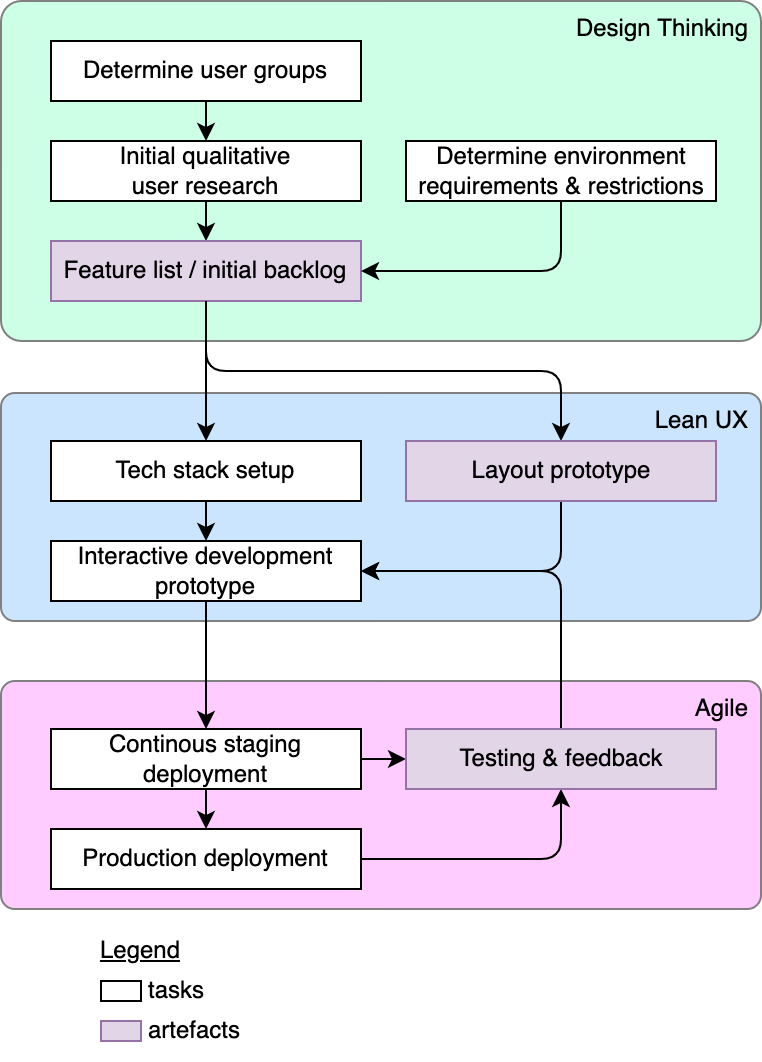
\includegraphics[width=0.8\linewidth]{pics/process.drawio.png}
  \caption{Software design process for the UI Editor.}
	\label{fig:process}
\end{figure}


% ---------------------------------------------------
% ----- Chapters of the template
% ----- for Bachelor-, Master thesis and class papers
% ---------------------------------------------------
%  Created by C. Müller-Birn on 2012-08-17, CC-BY-SA 3.0.
%  Freie Universität Berlin, Institute of Computer Science, Human Centered Computing. 
%
\chapter{Theoretical background}
\label{chap:background}

Before discussing the design and implementation of the UI editor, it is necessary to provide a brief overview of the applied parts of HCI and the specific context, challenges and Opportunities in which the UI editor was developed.
% 

\section{HCI}
Let me start by concretizing the HCI aspects and why this thesis approaches the area from an not so common standpoint.
\\
Many HCI books (e.g. \cite{Interactiondesign:2019ys} or \cite{LearnHCI:2020ys}) implicitly assume \label{def:Greenfield} Greenfield development,
which ''[...] is in its most distinct form when a new product is created from scratch – a new product or product platform, based on new technology, using new methodology [...]'' \cite{BrownfieldToGreenfield:2021ys}.
\\
While \cite[p. 392]{Interactiondesign:2019ys} for example mentions \textit{Environmental requirements} and \textit{Technical requirements} as part of the requirement discovery, the descriptions of these terms are more focused on physical limitations or user behaviours and technical requirements are mentioned only once and then not discussed further.
In contrast, I set my focus on the development inside a software company and an existing ecosystem, where resource, time and API limitations are present and existing users need to get productive with new software quickly.
\\
Thus, the user research phase started with collecting information about diffrent exisitng users as well as potentially new user groups the editor should target and adapting common HCI methods for qualtitative and quantitative user research like Moderated observations, interviews and questionaires.
I approached this phase with an open mind, recognizing that individual methods or applications of them might not be successful or don't provide value in this case study, but that much can still be learned from such experiences. As an example, after evaluation and test runs, I decided against Questionaires, because they showed less information content than other methods in this case study.
To align the methods with the projects goal and to select methods worthwhile trying from the large pool of user research methods, I used two systems:
\\
SMART criteria, which is a popular machanism to formulate goals and objectives that are clearly defined and also realistic to be implemented in time. \cite*{Atlassian:2021}.
I'll introduce them more in detail in chapter \ref*{chap:research}.
The second one are ''three major factors that an HCI designer should consider'' \cite[pp. 37-41]{LearnHCI:2020ys} according to Becker, which are
\begin{description}
  \item[Usability Factor] describes the spectrum from ''usable'' to ''unusable'' software. This is determined through the software design features implemented and how they help the user archieve their tasks in the environment provided.
  \item[Accessibility Factor] is high when as many users from different backgrounds can use the software in different enviornments. It includes, but is not limited to access for people with physical and other disabilites, as well as the entry hurdle a new user must overcome.
While it might look like this factor is not as important as the other two for specialized software mostly used internally, it should not be left out when designing and implementing. For example, even if currently no user with visual impairment is working with the software, it can always happen that an exisitng or new colleague suddenly has to rely on screen readers to continue his work.
  \item[Time-On-Task Factor] refers to ''[...] solutions that use up the appropriate of time to solve a problem.'' \Cite[p. 40]{LearnHCI:2020ys}. Obviously, to save users as much time as possible, a fast system is required.
But it is inevidable that the system, network delay and complexity of computation all have some minimal required time, and users understand that some operations might take time. More important is to reduce the perceived lag of interactions and give users feedback if a task takes longer to complete.
\end{description}
Evaluationg the outcomes of the research is at least as important as the research itself.
I experimented with diffrent ways to prepare and process the data to to present it more clearly as well as to consider different factors when discussing how to progress with the prototype.

\section{Project specific background}
To understand the usecase and value of the UI Editor, we first have to declare the fundamentals of the environment the editor will be embedded in.
The publishing houses resp. their digital departments (in the following \textit{customer}) purchase the license for an app or website (in the following just \textit{app}, as there is not much difference besides the end medium).
Then, they can import content via multiple ways into the system, or the editors write the content directly inside the tools provided as an Software-As-A-Service (SaaS).

\begin{figure}[h]
  \caption{Use Case diagram showing interactions from publishers, readers and frontend developers with the system}
  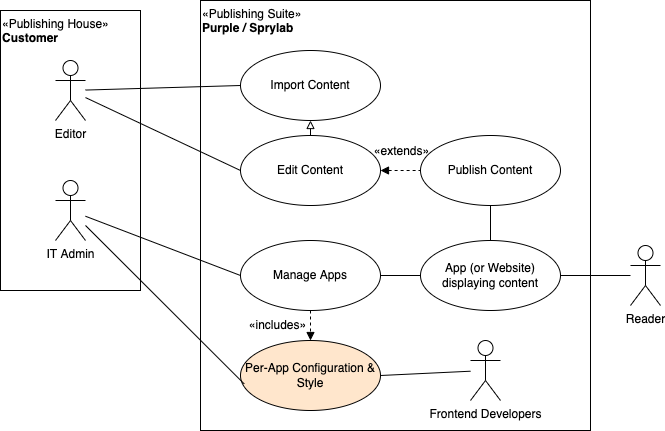
\includegraphics[width=\textwidth]{pics/purple-abstract.drawio.png}
\end{figure}

The UI editor fits into the Use case ''Per App configuration \& style'', with wich mostly Frontend Developers and Project Managers from Sprylab as well as some external customer's IT admins will interact. The goal is to lower the editing burden as much as possible, so that more of the configuration can be handed off to external customers while also improving usability for the developers of the company.
\\
Now that we have established a rough understanding of the environment and usecase the UI editor will be placed in, I want to explain more about the configuration and styling itself.
For that, it is important to understand the Frontend framework Sprylab uses for the delivery to apps and websites. It is called Purple Experience and is a Meta framework build ontop of Angular. The benefit is, that it is completely configurable via JSON files describing the routing, rendering of diffrent components,
connecting data sources (an API abstraction) with those components, loading assets like images and ads, and styling the whole page with CSS.
\\
These configs and assets are stored on an file system called \label{def:DynamicResources} \textit{dynamic resources}.
\\\\
Dynamic resources are individually managed and loaded for every app. This way, on mobile phones the endusers download an native core app, which in turn just downloads the dynamic resources and executes the angular app with the configs provided from the resources.
Similar, when a end user requests a website, the backend server just looks up the dynamic resources matching this app's Domain and renders the website using that config.
This way, all customers can share the same server instance(s), or at least don't require extra build artefacts per app.
\\
In addition, there are preview and live resources for every app, so that changes can be tested before they are released to the end users.
\\
If you have worked with larger, deeply nested JSON files before, you may recall that they get convoluted quite fast.
Also, manually handling ZIP files, changing assets and config files, packing everything back in a zip file and hoping one didn't introduce a typo anywhere is an inefficient an at times quite dangerous workflow.
\\
At Sprylab, there exists an tool called ''Storefront Editor'', which is used as the foundation for this new editor.
In the chapter \ref{chap:research} about User Research, I will outline the positive aspects and approaches which I reused for the new editor,
as well show the missing features and features the interview candidates noted as confusing, not working or slowing down their work.

The following UML sequence diagram displays a typical interaction of a user with the editor; pulling the current version, editing a file and merging the changes.
\textbf{TODO move to architecture?}
\begin{figure}[h]
  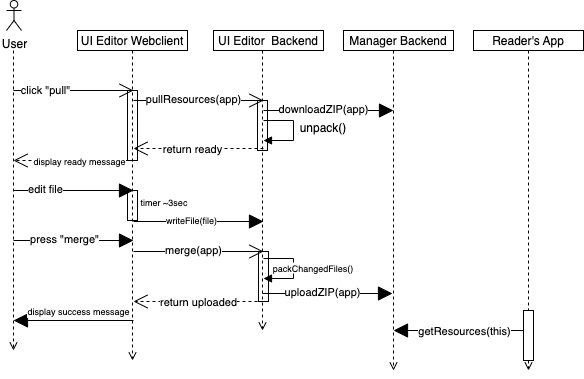
\includegraphics[width=\textwidth]{pics/user-flow.uml.drawio.png}
\end{figure}
% ---------------------------------------------------
% ----- Chapters of the template
% ----- for Bachelor-, Master thesis and class papers
% ---------------------------------------------------
%  Created by C. Müller-Birn on 2012-08-17, CC-BY-SA 3.0.
%  Freie Universität Berlin, Institute of Computer Science, Human Centered Computing. 
%
% TODO remove 2 - to use auto numbering
\chapter{User research and analysis}
\label{chap:research}


% Due to the limited size of the user group, the goal was not to gain <TODO> with high diversity of their demographics, but to have information saturation from fewer but more valuable insights into peolpe with diffrent workflows.

TODO maybe use this reference?:
\begin{itemize}
  \item \cite{Ross:2016} why companies dont conduct user research
\end{itemize}

Over ten years after the publication of Tomer Sharon's book ''It's our Research'', the listing of qoutes in the introduction about user research in software companies still feel as relevant as ever.
\\
''Yeah, but this study will delay our launch date.'', ''Yeah, but we can't learn much from only five participants.'', ''Yeah, but research sounds so academic.'' \cite[p. 4]{Sharon:2012mk} are only some of the statements that according to Sharon are often heard in software companies when discussing if UX research should be conducted.
\\
The common pressure from different stakeholders often leads to quick implementation of features and workflows without first investing time to figure the user's needs out, which may be faster in the beginning, but can badly impact the user's acceptance of the product due to cumbersome and slow workflows,
in the worst case leading to the user not using the product anymore.

To counteract this, it is crucial to conduct and evaluate user research methods, which is what I did for the development of the UI builder.

A starting point for qualitative user research is to define the goals through the help of the SMART criteria, which provide guidelines and formulated goals during research.

For the project, I defined the SMART criteria as following:

\begin{itemize}
  \item \textbf{specfic} - improve the workflow of users modifying dynamic resources for the Purple Experience.
  \item \textbf{measurable} - interviews after testing period concerning working speed, confidence and joy when editing resources, automated user tracking
  \item \textbf{assignable} - research and implementation will mostly be conducted by me, with input from CTO \& product owner, connections to external users through customer service team
  \item \textbf{realistic} - new software platform which reacts quicker, prvides more safety regarding errors and is scalable and extensible in the future. Limiting factors are time (as I only have three months for the first phase, including writinh this thesis)
  \item \textbf{time-related} - the new software should have at least the same feature set and be usable by company-internal users until the end of 2022
\end{itemize}

Remembering these points over and over again has helped me a lot when the focus on the actual goals was a bit unclear.
In addition, Becker (\cite[pp. 37-41]{LearnHCI:2020ys}) states that there are ''three major factors that an HCI designer should consider''.
Even though I couldn't find other publications mentioning them, they work well as additional guidelines to get broader research and product.
\begin{description}
  \item[Usability Factor] describes the spectrum from ''usable'' to ''unusable'' software. This is determined through the software design features implemented and how they help the user archieve their tasks in the environment provided.
  \item[Accessibility Factor] is high when as many users from different backgrounds can use the software in different enviornments. It includes, but is not limited to access for people with physical and other disabilites, as well as the entry hurdle a new user must overcome.
While it might look like this factor is not as important as the other two for specialized software mostly used internally, it should not be left out when designing and implementing. For example, even if currently no user with visual impairment is working with the software, it can always happen that an exisitng or new colleague suddenly has to rely on screen readers to continue his work.
  \item[Time-On-Task Factor] refers to ''[...] solutions that use up the appropriate of time to solve a problem.'' \Cite[p. 40]{LearnHCI:2020ys}. Obviously, to save users as much time as possible, a fast system is required.
But it is inevidable that the system, network delay and complexity of computation all have some minimal required time, and users understand that some operations might take time. More important is to reduce the perceived lag of interactions and give users feedback if a task takes longer to complete.
\end{description}

\section{Identifying and categorizing users and user groups}
\label{sec:user-groups}
In order to effectively design and implement the UI editor, it is crucial to understand the needs and preferences of the various users and user groups who will be using the tool.
Therefore, the first step in the user research process was to identify and categorize the different users and user groups who will be using the editor.

In a later section (\ref{sec:personas}), I'll build concrete Personas for the different user groups utilizing the information gained from the interviews.
\\
Because we already have existing users that work with the previous editors and other tools from the ecosystem, it was relatively easy to collect a list of internal and extneral users, which either I personally knew or I could write a short message asking about if and how they use existing tools and modify dynamic resources.
I see that this won't be as easy when dealing with a larger user base or primary external customers, when this first step probably requires more effort to collect a user overview upfront.
\\
With a list of many of the users, I started grouping them to understand the characteristics and needs of each user group, through which can ensure that the UI editor is tailored to their specific requirements and can be used effectively by all users\footnote{When I refer to ''all users'', I mean the group of users that are expected to work with the tool. There is an expected technical and domain specific base knowledge that the Editor won't cover in it's initial form}.
\\
I derived the follwoing common factors from the users, which made the communication and categorization a lot easier.

\begin{itemize}
  \item \textbf{quantitative usage} There were users who relied on the tools for most of their work, while others like the external customers accessed the tool a few times a year.
  \item \textbf{common tasks} I roughly categorized the common tasks into three groups:
    \subitem \textbf{Heavy configuration} Mostly internal devs used the tools to build new apps and websites from scratch (or derived from exisiting apps), making many modifications, from structural changes to the seperate views, menus, data sources and more, over styling and translating messages to diffrent languages.
    \subitem \textbf{Moderate configuration} Project devs and customer support people copy resources from existing apps and adapt them for new brands, which often includes changing colors and logos, adapting texts or switching authentification flows.
    \subitem \textbf{Small changes} External customers often only use the tools to exchange some ads, translations or logos, which affects a small set of files.
  \item \textbf{expertise} 
  %<kann man bei schlechter software gut erkennen, leute mit viel erfahrung checken sachen, aber ist für neue nicht intutitiv>
    \subitem \textbf{Technical} Depending on the area of education and working time in the web development industry, the expertise about web technologies, languages like CSS and JSON and often also intuition differs between users.
    \subitem \textbf{Domain- and Platform Specific} There is a lot of vocabulary, functionality of the Purple Experience and other systems as well as permutations of configurations that users learn with time.
\end{itemize}

% ... more
\section{Qualitative user research}

The existing user base enabled me easy access to subjects for qualitative user research methods.
Using one or multiple ways of Triangulation \cite[p. 264]{Interactiondesign:2019ys} can strengthen the significance of the research outcome. Limitations of a method or source can be removed by variation of those, resulting in a less distorted picture.
Therefore I used metholodical triangulation (using multiple data gathering techniques) as well as triangulation of data (collecting data from different people and different sources).
Moderated observations combined with interviews proofed to be a good fit for this case study, as they are interaction driven and the observer can react directly on behaviours / emerging topics and steer the process.
This stands is contrast to more passive methods I found like passive observations or user recording and tracking analysis, where the outcome only depends on the
prepared question / task and the users behaviour and which can't adapt to changed circuumstances etc. during the application.
\\\\
The chosen structure for the observations and interviews looks as following:

\begin{description}
  \item [Introduction (ca. 5min)] used to explain the circuumstances and the goal of the session, how we proceed, which data I will collect and how I will evaluate the data afterwards.
  \item [Moderated Observation (10-15min)] have the observed perform specific tasks in a prepared environment
  \item [Semistructured Interview (ca. 15min)] ask prepared questions as well as open ones and discuss observation situation
\end{description}
Interviews followed observations to discuss issues encountered during the moderated observation and to gain deeper insight into the workflow and potential problems.
\\
As I had no prior experience conducting these methods with a scientific approach, it was important to me to test the whole process before scheduling all the other meetings. One of our working students agreed to be a test candidate and we went through the tasks and questions I planned, after which he gave me feedback.
Testing the methods and specific questions before conducting them on a broader audience helped finding questiones that were ambiguous or lead to a lot of repetition of already known facts. For the moderated observation tasks it gave me feedback on the difficulty and time they would take for others on average, which tasks needed clearer formulations and which were already good.
\\
In total, I performed the user research on six persons, from which one was an core Purple Experience developer, two were working students from our project department, one was an developer from an different department who had worked with the software some time prior, one Customer Support Manager from our company and one external user from an publisher.
\\
TODO: SME (subject matter expert) (ref. ABOUT FACE - The essentials of interaction design) ''authorities on the domain on which the product will operate. This is of critical importance in domains that are highly complex or very technical.'' p.41

\subsection{Moderated observation}
\label{subsec:modobs}
I prepared a list of six tasks, with the last two beeing optional depending on the time left and the confidence of the user with the platform I perceived during the beginning.
That way I could present the same first tasks to every interviewee regardless of their level of knowledge, and present the last two tasks if we had enough time left.
Also, it was important that the tasks did not build on each other to prevent the observed person getting stuck because of an earlier mistake.
To me, it was more important to see a variety of tasks getting performed than one task beeing executed without errors. 
\\
In practice, I prepared an example app on our staging system, noted the link down and downloaded the initial state so that I could easily reset the enviornment after each observation.
The six tasks were
\begin{itemize}
  \item Change english app menu entry "Newsstand" to "Home" on all platforms (Web, Android and iOS)
  \item Change the Advertisement banner target on top of the home page to https://google.com 
  \item Change the exnglish text "Latest Issues" on the home page to "Read new Issues"
  \item Change color of "Read new Issues" and "Latest Articles" headers on the home page to the app's primary color.
  \item \textit{(Optional)} Add an dropdown on the home between "Read new Issues" and "Latest Articles"
    \subitem It should show all publications connected to the app
    \subitem It should set an URL parameter ''publication'' to the id when selected
    \subitem Define the reset message as ''All publications''
  \item \textit{(Optional)} Configure the filter of the ''Latest Articles'' list to only show articles from that publication
\end{itemize}

These were constructed in a way that I anticipated some errors so I could see how users tried to figure out what went wrong and fix them.
These cases then also occurred, for example the first task was often only done for one of the three platforms, the ''Latest Issues'' text was not found in the translation files or
the wrong CSS selector was used to recolor the header elements on the home page, leading to more elements beeing recolored.

The optional tasks were presented to four people, of which three solved them at least one of them successfully, only the core developer solved all six tasks completely.
With the consent of the interviewees I recorded their screens during the observation to rewatch specific actions or flows if required.
\\
TODO: noticed workflow patterns that can be improved? like file opening, switching files (quick links \& file tabs)

\subsection{Interview}
\label{subsec:interview}
For the interview, I chose a semistructured interview as the appropriate tool. The interviewer has a list of open and closed questions, through which he can ensure that important topics are coveredw hile also allowing for flexibility to delve deeper into specific issues and ideas that may arise during the interview.
\\
My prepared questions consisted of some closed questions, like how often they interact with the tools, how confident they feel implementing changes or fixing errors, as well as some open questions like to describe step by step what the most recent task was they performed with dynamic resources, how they were onboarded etc.
Then, if I had notices points during the observation, I addressed these points directly, else I directly introduced the open question ''If you dream of the UI builder, <>, how would it look like, which features would you expect and what workflows are most important to you?''.
\\
The semistructured interviews proved to be valuable in providing insight into the experiences and needs of the users. Through the interviews, I was able to gather a lot of new ideas and saw how different features were massively valued differently by the users. Two of the interviewees even provided written lists of their ideas and suggestions which they sent me afterwards. After every interview (wich I also recorded), I filled out a Word document noting basic questions about the person and it's usage of the dynamic resources, important situations from the observation, input from the interview and linked to the recordings in case I needed to rewatch parts of it.
\\\\
Some of the outcomes were:
\begin{itemize}
  \item The way users validate their changes differs widely, some use a preview window in the old editor, some merge changes into the resources and view it on the website or inspect the app's javascript context, some prefer seperate windows, some embedded frames to see code and preview at the same time.
  \item Rearranging or adapting the layout of the tools / editor to match the current screen and browser window size is important, e.g. hide unecessary panes if not used, make the window the user currently works in larger to see more content at once.
  \item Editing multiple files at once (in the old editor one could only edit one file at a time, had to close the current and open the next one).
  \item Colaborative working: Seeing the current state of the resources, e.g. if a live or preview resource is processing, if other users are working in the same app parallel, and having git-like line-by-line diffs of the changes made.
\end{itemize}

Some of these points and their implementations will be covered in chapter \ref*{chap:prototyping} \ref*{chap:impl}.

\section{Quantitaive user research}

In the initial stages of research, the use of questionnaires was considered as a method of gathering information from existing and potential users.
However, as the outcome of the qualitative research was already productive, it proved difficult to design a questionnaire that would provide additional information while adhering to common design rules for questionnaires in terms of length, number of questions, and type of questions.
While prototype questionnaires were created using Microsoft Forms, I found them to be too long, difficult to understand, or not relevant to the development of prototypes.
Therefore, it was decided to rely solely on qualitative research results for prototyping and feedback, along with some automatic tracking implementation (See TODO squeaky ref).
\\
\section{Process and visualize the outcomes of the initial user research phase}

To gain as much value from the raw research data it is crucial to find some methods to process and visualize the outcomes.
A common approach at companies is to write ''tickets'' in their ticket system of choice, in case of Sprylab Jira (\url{https://www.atlassian.com/de/software/jira}).
From my experience, Jira and co. proof valuable once the development process itself started and the state of the tasks must be tracked.
But for discovery and prioritization of features, scrolling through lists of tickets with different priority levels, where then the tickets in the lists are sorted differently again, does not allow a good overview of effort and benefit of each feature.
Thus, based on the condensed notes from the observations and interviews I tried out two alternative ways to figure out different features and how they can be prioritized.

\subsection{2x2 Opportunity Matrix}

This two-dimensional vizualization of a set of proposed features prooved helpful when prioritizing tasks with other stakeholders,
as it shows the (approximated) cost of implementation as well as the value the feature can have for users.

The matrix I used is a slightly modified adaption from \cite[p. 181]{LearnHCI:2020ys}, replaced the term ''idea originality'' on the x-axis with ''Value''.

\begin{figure}[h!]
	\centering
  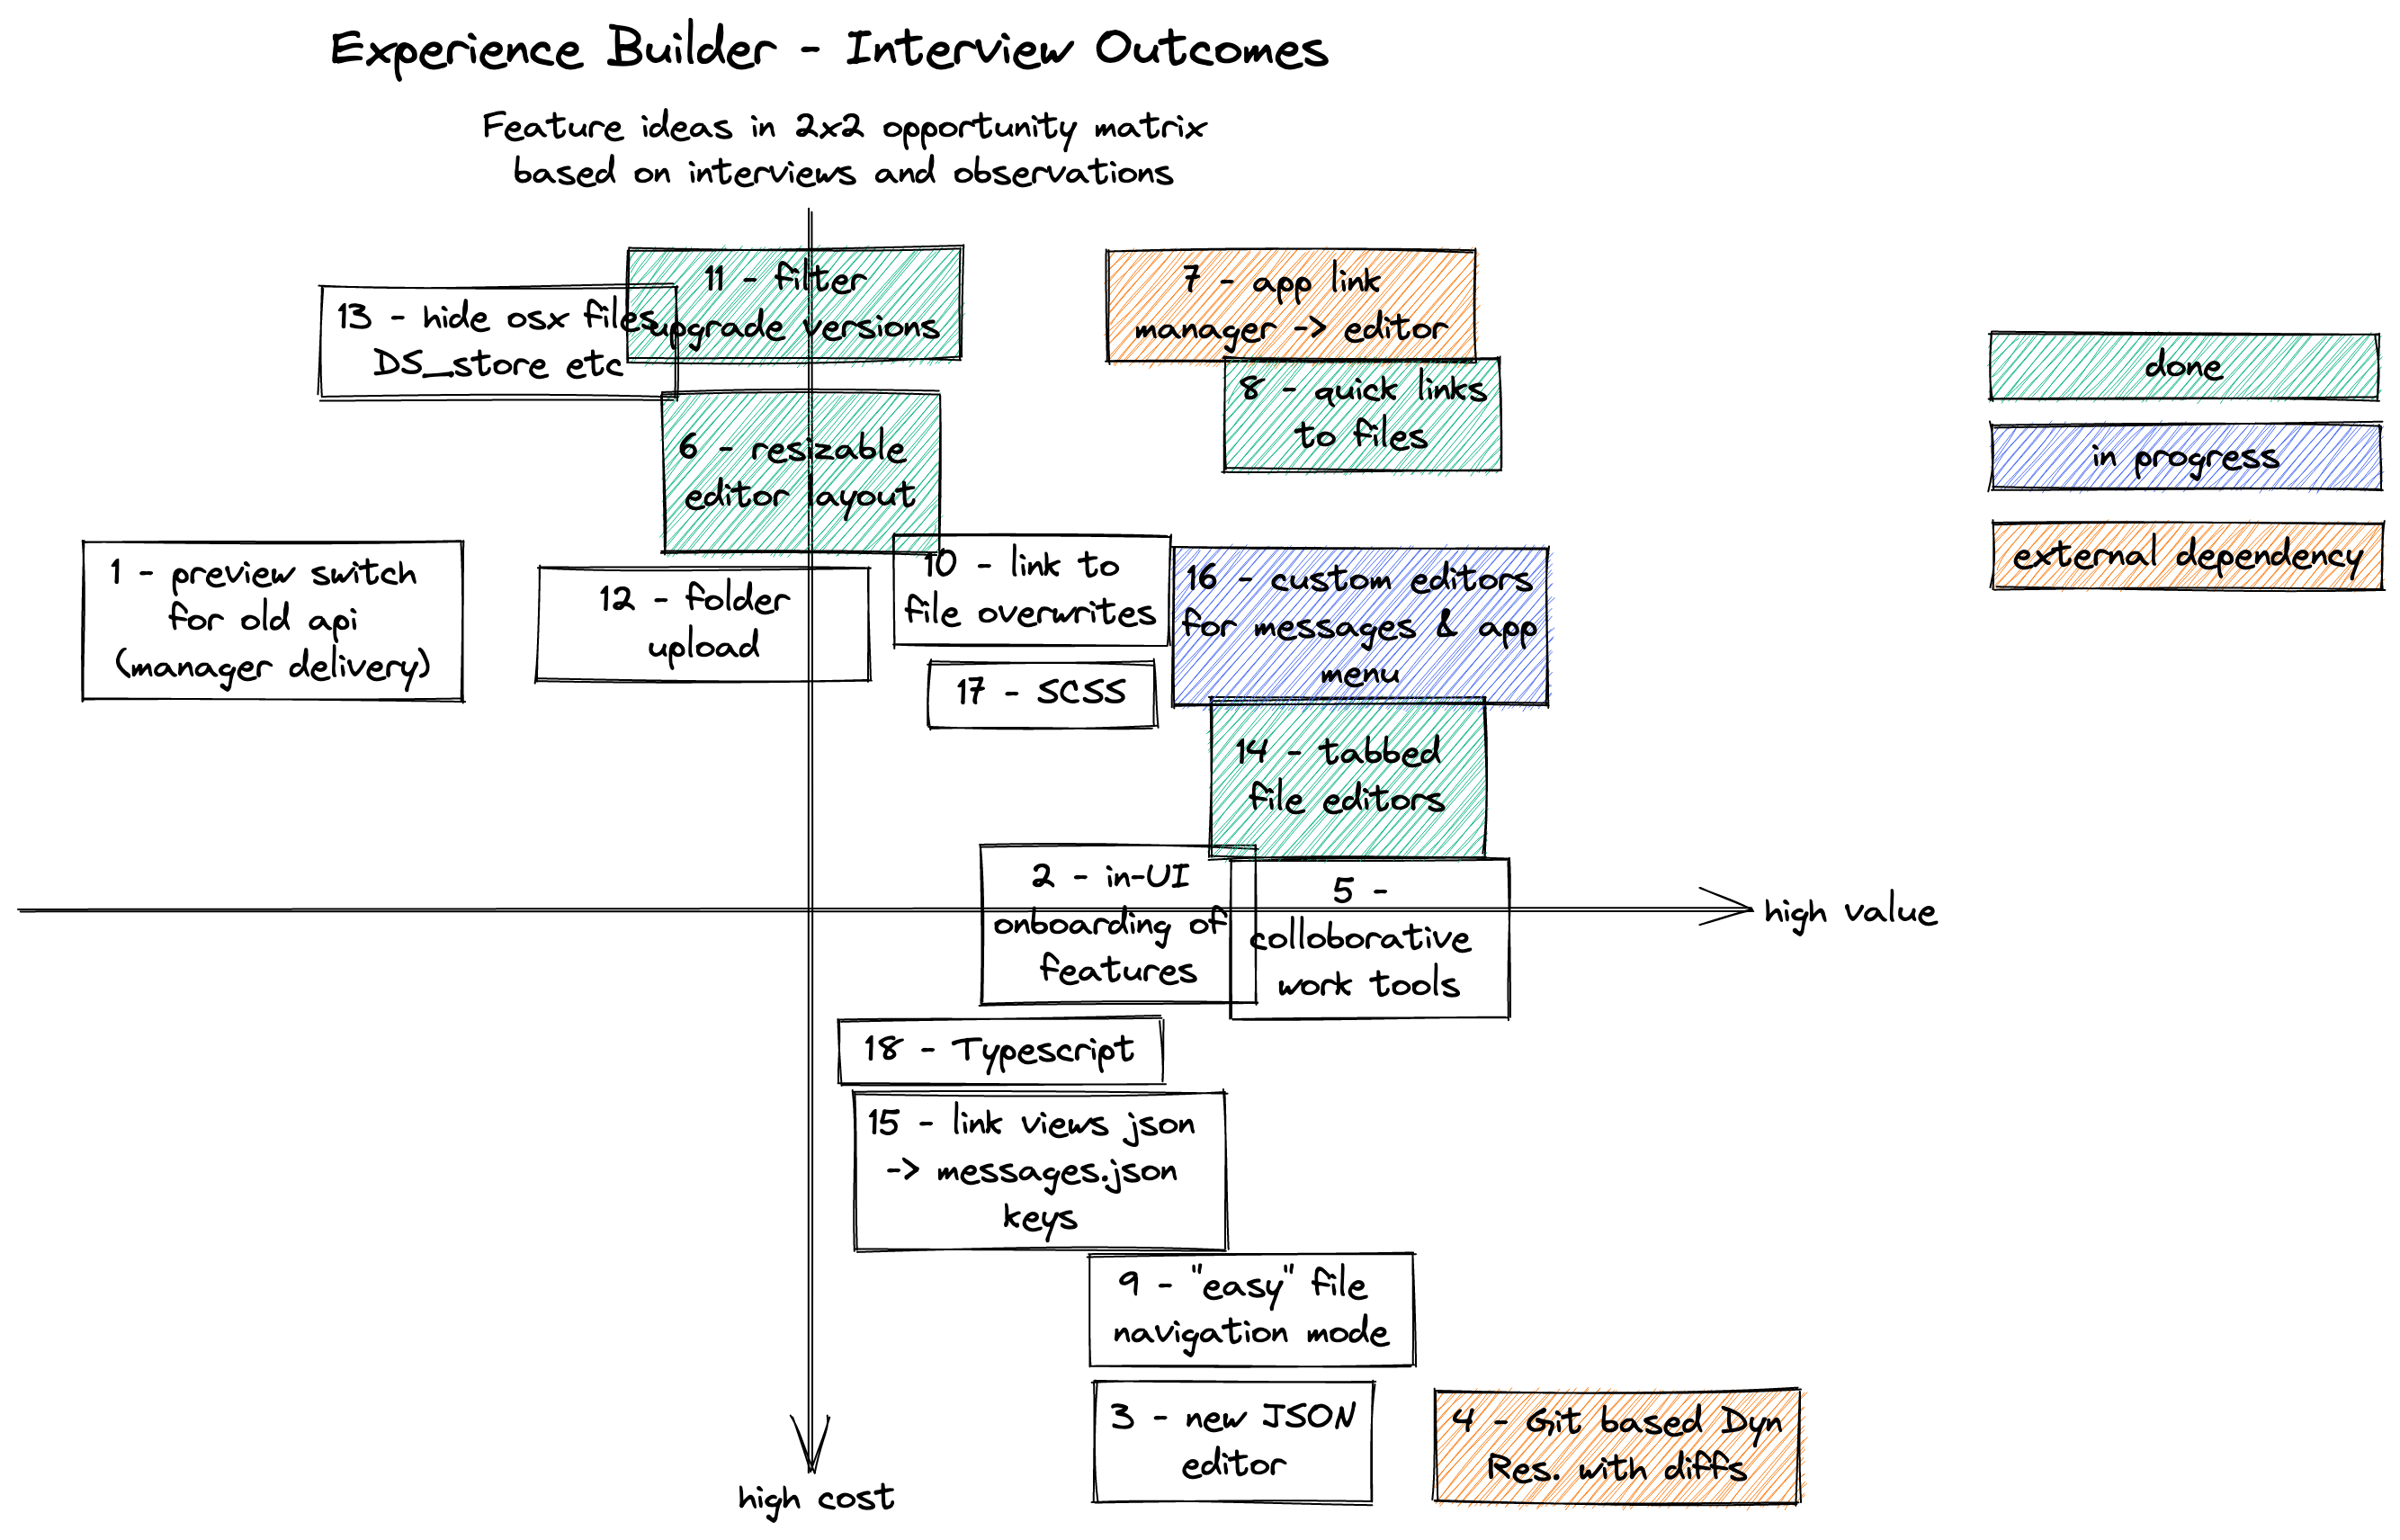
\includegraphics[width=\textwidth]{pics/feature_cost_matrix.excalidraw.png}
	\caption{2x2 Opportunity Matrix during the early phases of development}
	\label{fig:opportunitymatrix}
\end{figure}


\section{Building Personas}
\label{sec:personas}

TODO: move to appendix?

Personas are descriptions of fictional users of the product, incorporating assumptions and optinally data for a user group.
They aim to give developers and designers more context and depict real potential users, which makes it easier for a developer to empathize with the user.
The following three Role-based Personas are derived from \ref{sec:user-groups} and the outcomes of the interviews, based on the description of Personas in \cite[pp. 403-405]{Interactiondesign:2019ys}
\\
\hrule
% Persona 1
\subsection{John - Purple Expeirence Product Developer}
\label{subsec:persona:productdev}
\subsubsection{Background and Skills}
John (34) is a senior Angular Web Developer at Sprylab, working there for two years. He was born in Berlin and lives in Lichterfelde with his wife and mostly works from home. He is passionate about Angular, Typescript and Developer Experience in general, studied Computer Science at the Beuth Hochschule and hosts Angular conferences.
\\
\subsubsection{Goals and work with the Editor}
\begin{itemize}
  \item Test newly developed features and the related configurations
  \item Configure test apps for development and QA purposes
  \item Support in case Project Developers like <TODO> encounter problems
  \item John works with the editor multiple times a week
\end{itemize}

\hrule
% Persona 2
\subsection{Steffi - Project Developer}
\label{subsec:persona:projectdev}
\subsubsection{Background and Skills}
Steffi (23) studies media informatics and works as a working student at Sprylab since a year. This is her first job in the industry and she is learning new things every day. Her skills include writing CSS and understanding modern web technologies, but she still struggles using native and custom debugging tools if something goes wrong.  
\\
\subsubsection{Goals and work with the Editor}
\begin{itemize}
  \item Configure new apps based on existing templates and adapt them to customer's requirements
  \item Add new components or change data sources for existing apps
  \item Add custom HTML pages or Javascript snippets to intergrate external services
  \item Change styles, color schemas or icons when a customer has a rebranding
  \item Steffi uses the editor as a primary tool for her work
\end{itemize}

\hrule
% Persona 2
\subsection{Karsten - IT department at a publishing house}
\label{subsec:persona:itpublishing}
\subsubsection{Background and Skills}
Karsten (46) worked in the publishing industry for 20 years, but only during the last years his company, aga magazine publisher, tries to catch up with the digital development and trends. He is still struggling with his role and is thankful for every trick or tool that makes his life managing the digital products easier.
\\
\subsubsection{Goals and work with the Editor}
\begin{itemize}
  \item Exchange logos and colors when the magazines he supervies get a redesign
  \item Add new ads to different views when a new campaign starts
  \item Manage URLs to external sites when they change
  \item Karsten uses the Editor once a month on average
\end{itemize}

% !TeX root = ../thesis_main.tex

% ---------------------------------------------------
% ----- Chapters of the template
% ----- for Bachelor-, Master thesis and class papers
% ---------------------------------------------------
%  Created by C. Müller-Birn on 2012-08-17, CC-BY-SA 3.0.
%  Freie Universität Berlin, Institute of Computer Science, Human Centered Computing. 
%
% TODO remove 2 - to use auto numbering
\chapter{Prototyping}
\label{chap:prototyping} 

After collecting the inital user feedback, I started drawing minimal digital ''paper'' prototypes using Figma to gather vizualizations of the proposed UI layouts.
Two ideas emerged from the interviews: a (file-)editor-centric layout and a preview-centric layout.
\section{Editor centric vs preview centric layout}
The editor-centric layout is inspired by modern text editors / IDEs like VS Code (\url{https://code.visualstudio.com/}), which was mentioned as reference during the interviews multiple times.
There, the central pane is the editor for the currently open file, while on the sides additional panes for file management, preview and more can be shown.
The familarity, especially to developers who are used to IDE layouts, could help new users adopt patterns to work with the UI they use in other tools as well.
\\\\
The idea for a preview-centric layout was inspired by popular generic website builders like \url{https://wix.com} or \url{https://wordpress.com}, where the user
can see the page in an interactive mode, move, configure or place elements, and then has on the side additional panels like one with information \& options about the
currently selected element.
There are also framework-agnostic tools like \url{https://vwo.com/why-us/technology/visual-editor/}, but they either focused more on only editing the style and not the structure of the page or were not
compatible with the Experience's framework and data format. 
\begin{figure}[h]
  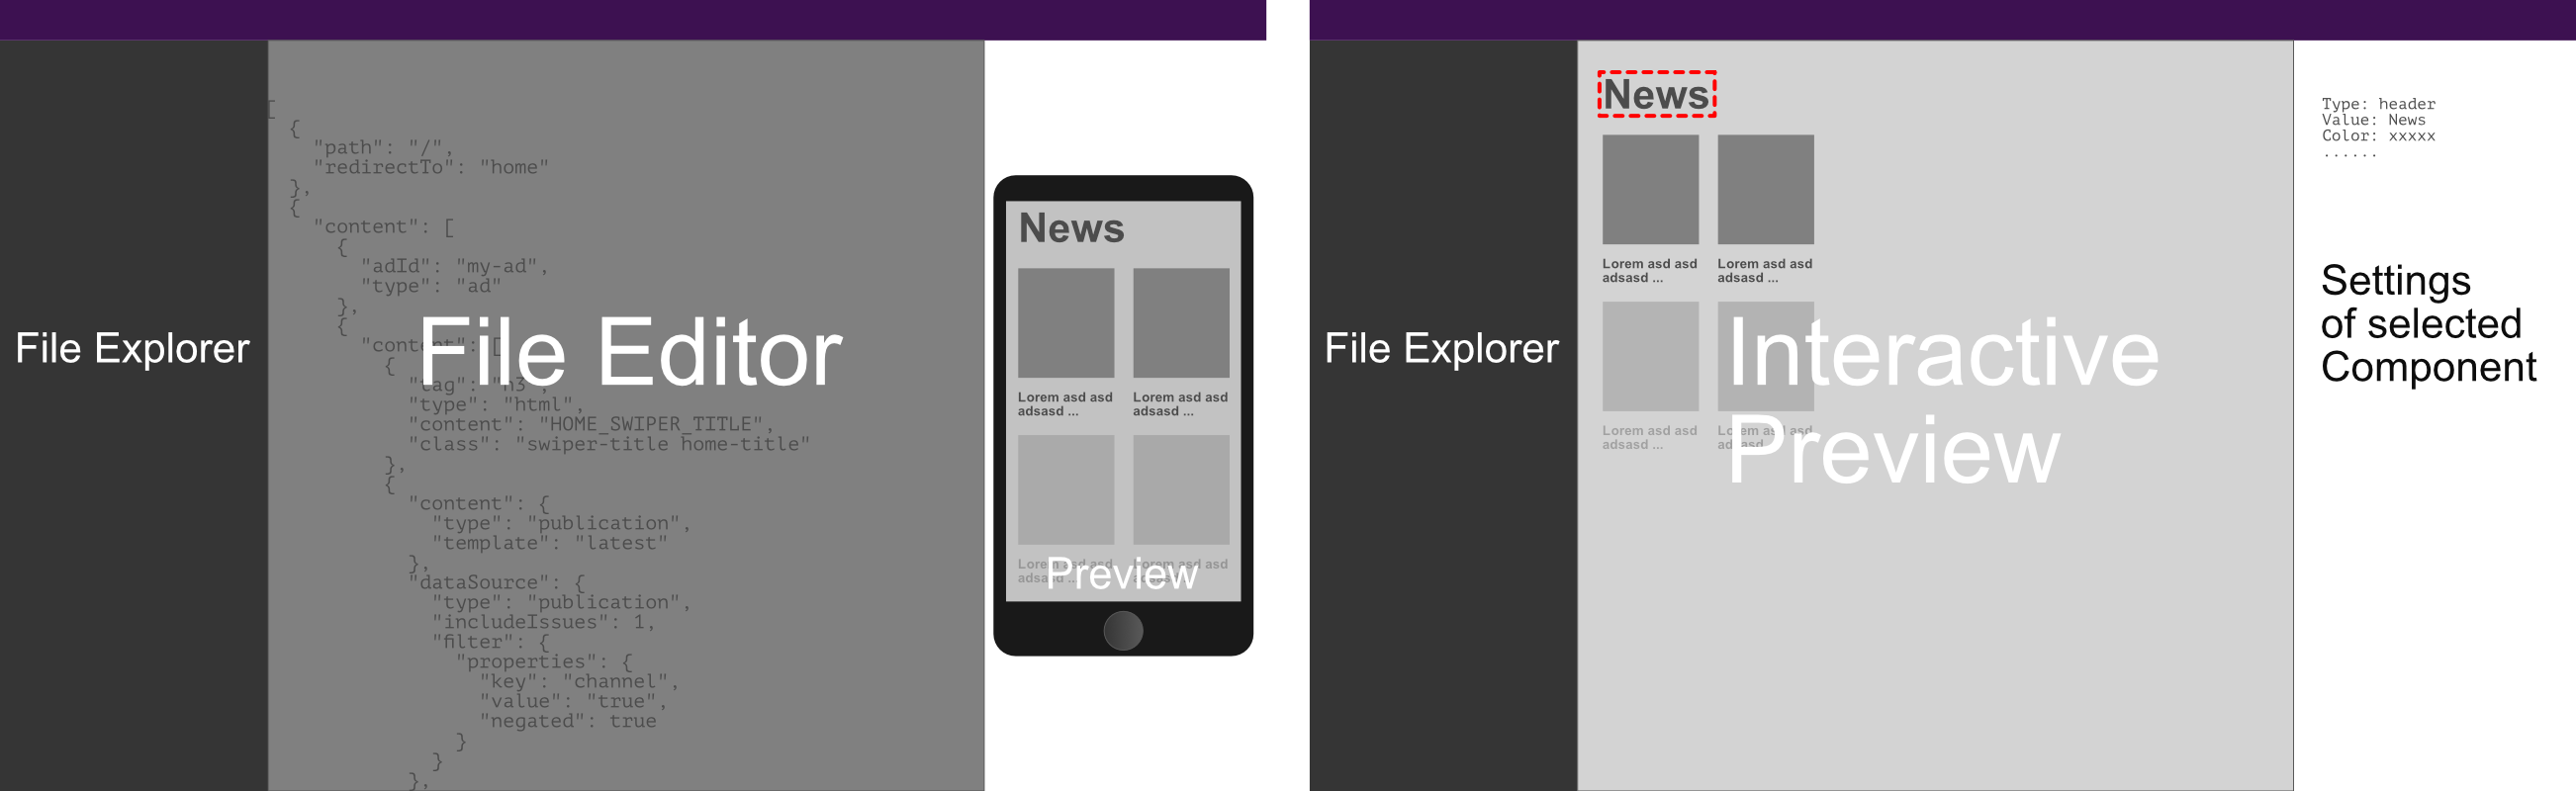
\includegraphics[width=\textwidth]{pics/editor_centric_vs_preview_centric.png}
  \caption{Mockups: Editor centric vs preview centric editor layout}
\end{figure}
Ultimately our choice fell to the editor centric layout, the following are some of the reasons for it over the preview-centric one:
\begin{itemize}
  \item The configuration structure of the Experience framework was not built with preview-based editing in mind, causing many functionalities to be hidden and invisible to the user, making it difficult to reproduce specific conditions in the editor environment.
  Thus, editing in a preview-centric mode could lead to more confusion for the editors than speeding up the process.
  As the configuration schemata are mostly fixed, it was deemed that preview-based editing would not be suitable in this case.
  \item After evaluating available libraries and examples, we concluded that building a reliable and usable preview-centric editor is more complicated and uncertain to result in a viable product within the limited time frame of this bachelor thesis.
  For editor-centric UIs, many third-party libraries exist that can be integrated into the UI, such as Microsoft's Monaco Editor (\url{https://microsoft.github.io/monaco-editor/}) for editing generic web-related files with automatic syntax highlighting and error detection, and JSON Editor for working with JSON configurations with provided schema.
  \item The user base consists mostly of tech-affine people who are used to layouts of IDEs, and the old tool also had a similar editor-centric layout.
  As Jakob's Law of the Internet User Experience states, the user's understanding of a website is directly tied to their mental model of that system \cite{Nielsen:2000} and \cite[p. 2]{LawsOfUX:2020ys}. Introducing an unconventional workflow comes with the danger of confusing the user, causing mistakes, and potentially leading to dissatisfaction with the tool.
 
\end{itemize}


% !TeX root = ../thesis_main.tex

% ---------------------------------------------------
% ----- Chapters of the template
% ----- for Bachelor-, Master thesis and class papers
% ---------------------------------------------------
%  Created by C. Müller-Birn on 2012-08-17, CC-BY-SA 3.0.
%  Freie Universität Berlin, Institute of Computer Science, Human Centered Computing. 
%
% TODO remove 2 - to use auto numbering
\chapter{Implementation and deployment}
\label{chap:impl} 

The phase of implementation and deployment followed an agile development process where changes could be deployed easily to get fast feedback from users.

% \localtableofcontents

\section{Architecture}

Let's start with an overview about the architecture and high level user flows.
We have three software components relevant for a basic interaction with the system: the editor frontend, the editor backend and the ''Manager'' backend, which is responsible for
authentication, app management and providing the dynamic resources in an ZIP format.
At the beginning of a user journey, the user visits the root domain (e.g. \url{https://builder.purplemanager.com} for production apps) and logs himself in.
The authentication details will not be covered here as these would go beyond the scope of a bachelor thesis and are not relevant for the UX.
The API the \Gls{manager} exposed and the way dynamic resources get downloaded and merged is one of the basic technical requirements introduced by the surrounding ecosystem.
\\
The UML sequence diagram fig. \ref{fig:userflow} displays a typical interaction of a user with the editor frontend after he selected an app; pulling the latest dynamic resources, editing a file and merging the changes.
\begin{figure}[h!]
  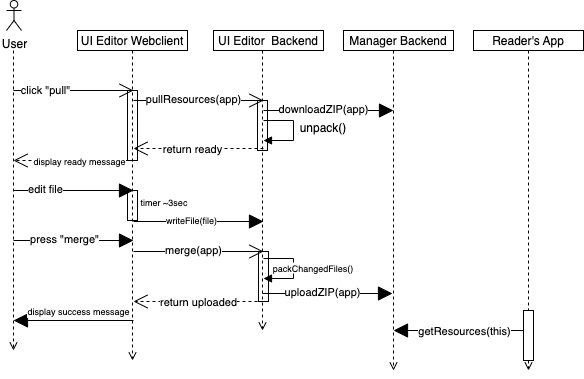
\includegraphics[width=\textwidth]{pics/user-flow.uml.drawio.png}
  \caption{A typical interaction of a user with the UI Editor frontend and it's dependencies}
  \label{fig:userflow}
\end{figure}
\pagebreak
\section{Software stack}
From a company's perspective, it is advantageous to keep the technology stack as narrow as possible.
For this case study, the most important point was the availability of additional personnel with knowledge about the frameworks and languages used.
To conform with the company's \Gls{devops} practices the application only requirement is to be able to run inside a Docker container in a Kubernetes environment.
\\\\
For this project the Typescript language (\url{https://www.typescriptlang.org}) is used on back- and frontend.
The advantage is the availability of many skilled personnel in the company as well as an established ecosystem and easy sharing of code and type definitions between frontend and backend.
\\
The rest of the software stack is fairly common in todays web development industry too:

\begin{description}
  \item[Frontend] \leavevmode
  \begin{description}
    \item[Rendering framework] \textit{React JS v18} (\url{https://reactjs.org/})
    \item[UI Component Library] \textit{Blueprint JS} (\url{https://blueprintjs.com/}) provides components so we can rely on a consistent design system with common functionality like buttons, dropdowns, filters etc. already implemented.
    \item[Other libraries] \textit{ReactQuery / TanQuery} to manage, cache and invalidate HTTP API requests to the backend, \textit{Zustand JS} for shared reactive state management and \textit{Zod} for type validation at runtime.
  \end{description}
  \item[Backend] \leavevmode
  \begin{description}
    \item[HTTP Server] Express on Node JS, which is the most common combination to run an Javascript based HTTP server (see \cite{Github:VanoDevium/node-framework-stars}).
    \item[Routing abstraction] TSOA (\url{https://github.com/lukeautry/tsoa}) on top of Express, which is a Typescript library to provide Java-Spring like syntax with controllers, dependency injection and parameter validation at runtime.
  \end{description}
  \item[Testing] using Vitest (\url{https://vitest.dev/}) for Unit tests and Playwright (\url{https://playwright.dev/}) as E2E test runtime. 
  \item[DevOps] Gitlab Pipelines to build, test and package on every merge request or commit to develop and master branch.
  \item[Project Setup] Monorepository with PNPM as package manager and Turborepo to manage package dependencies and automatic optimal build scheduling and caching.
\end{description}

\section{CI/CD}

Continuous Integration and Continuous Delivery, short CI/CD, a core practice of agile software development, enables fast release and deployment cycles which is crucial for agile prototyping and development.
A Gitlab CICD Pipeline was set up for the UI builder, consisting of Build, Package, and Deploy stages.
The Build stage also executed unit and end-to-end tests due to technical reasons for efficiency.\\
Having a fast and reliable CI/CD process during development and prototyping was valuable, as it allowed for quick reactions to user input and deployment to a staging domain for user feedback in under 10 minutes.
Separating staging and production systems also allowed for more confident deployment of quick fixes for validation in a production-like environment without interrupting users.

\section{Feature examples}

In the following section, a selection of features is presented that were implemented during the UI Editor case study.
These features are chosen as examples to how the HCI methods and outcomes from the user research phase influenced their design and how they can improve the user's experience with the tool. 

\subsection{File management - open multiple files as tabs}

A common workflow consists of editing multiple files at the same time, for example having the view configuration open while adding translations for newly added components.
The old editor tool only allowed to open one file at a time and get closed when the user opened another one. This showed up as a big slowdown during the moderated observation.
All interview subjects mentioned they have to work on multiple files and that they are annoyed by the workflow, especially when opening large view configs can take more than 30 seconds.
\\
The solution was inspired by the file management that most IDEs provide, a bar on top where all the opened files are listed and the user can quickly switch between them or close the ones he doesn't need anymore (see fig. \ref{fig:file-tabs}). 

\begin{figure}[h]
  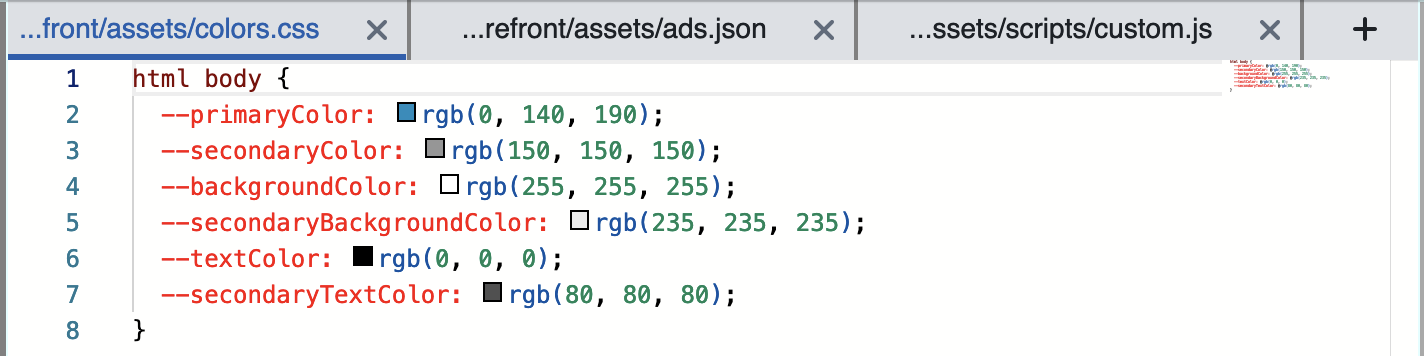
\includegraphics[width=\textwidth]{pics/file_tabs.png}
  \caption{Screenshot of the latest iteration of file tabs}
  \label{fig:file-tabs}
\end{figure}

\subsection{File management - quick links}

A second feature regarding the file management are so called ''quick links''. While all target groups benefit from this, especially for the personas \textit{Steffi, \ref{subsec:persona:productdev}} and \textit{Karsten, \ref{subsec:persona:itpublishing}}
this can speed up common tasks considerably.

The basic idea is to bookmark commonly used files, e.g. the translation or ad config, and have them prominently available when opening a new app.
For the implementation, three factors needed to be considered:
\begin{description}
  \item[Where to save?] The quick links are stored in the \Gls{localstorage} of the user's browser, so the list is available across apps.
  \item[How to manage?] Currently, the user has a list on the settings view, where he can add or delete new entries, but has to enter the file path manually.
  A proposal already exists to either add a file picker in the settings or add a bookmark button to the file manager on the primary editing view.
  \item[How to present the links?] The links must be easily accessible to provide the intended benefit. The solution was to show them when entering the \textit{edit} view and no file was opened yet.
  In addition, the UI shows if the link points to a file, which gets opened as a new file tab, to a folder which will navigate the file explorer to there, or if the path doesn't exist in the current app.
  \begin{figure}[h!]
    \centering
    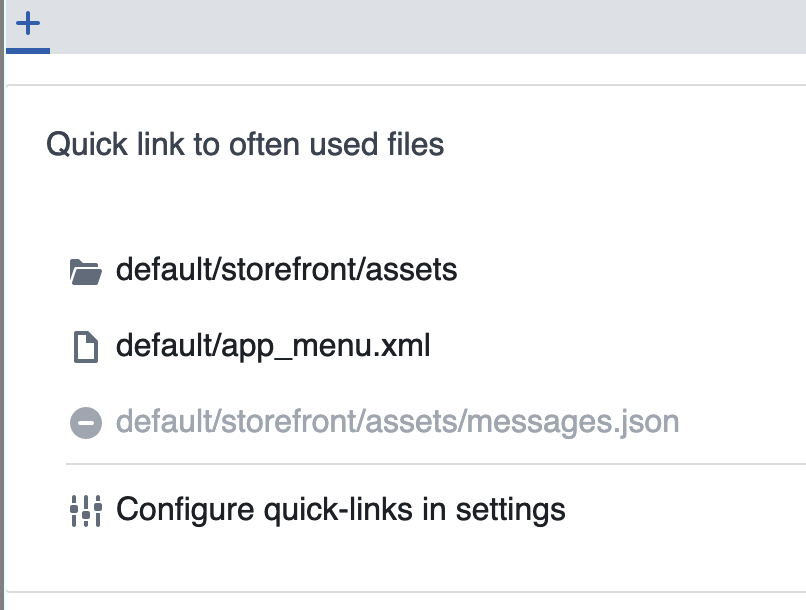
\includegraphics[width=0.4\textwidth]{pics/quick_links.png}
    \caption{The three types of quick links: Folder, file and not available}
  \end{figure}
\end{description}

\subsection{Editor - Abstraction to provide per-file custom editors}

Purple Experience relies on a variety of configuration files, all with different schemata and functional intents.
To provide an efficient and error reduced workflow to users, it is important to have specialized file editors.

For view configurations for example, we utilize the JSON Editor Library (\url{https://github.com/json-editor/json-editor}) combined with the generated JSON Schema files,
for the translations we have a custom editor that has a fuzzy search function and makes it easy to manage translation entries.

The abstraction is done solely in the frontend and follows React's "\Gls{comp-over-inh}" pattern.
To add a new specialized editor the only two steps are creating a new functional component that implements the \textit{EditorImpl} interface
and add that editor in the \textit{EditorRegistry} to get returned for the file paths in question.

\begin{figure}[h]
  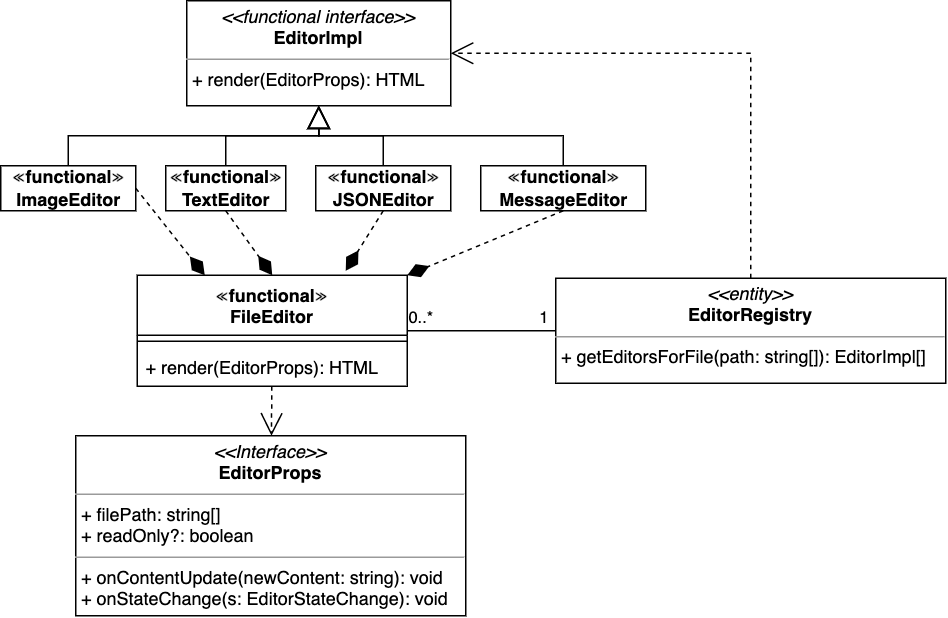
\includegraphics[width=\textwidth]{pics/abstract_editor_uml.drawio.png}
  \caption{Class diagram showing the editor abstraction in React JS}
  \label{fig:abstract-editor}
\end{figure}
\begin{figure}[h]
  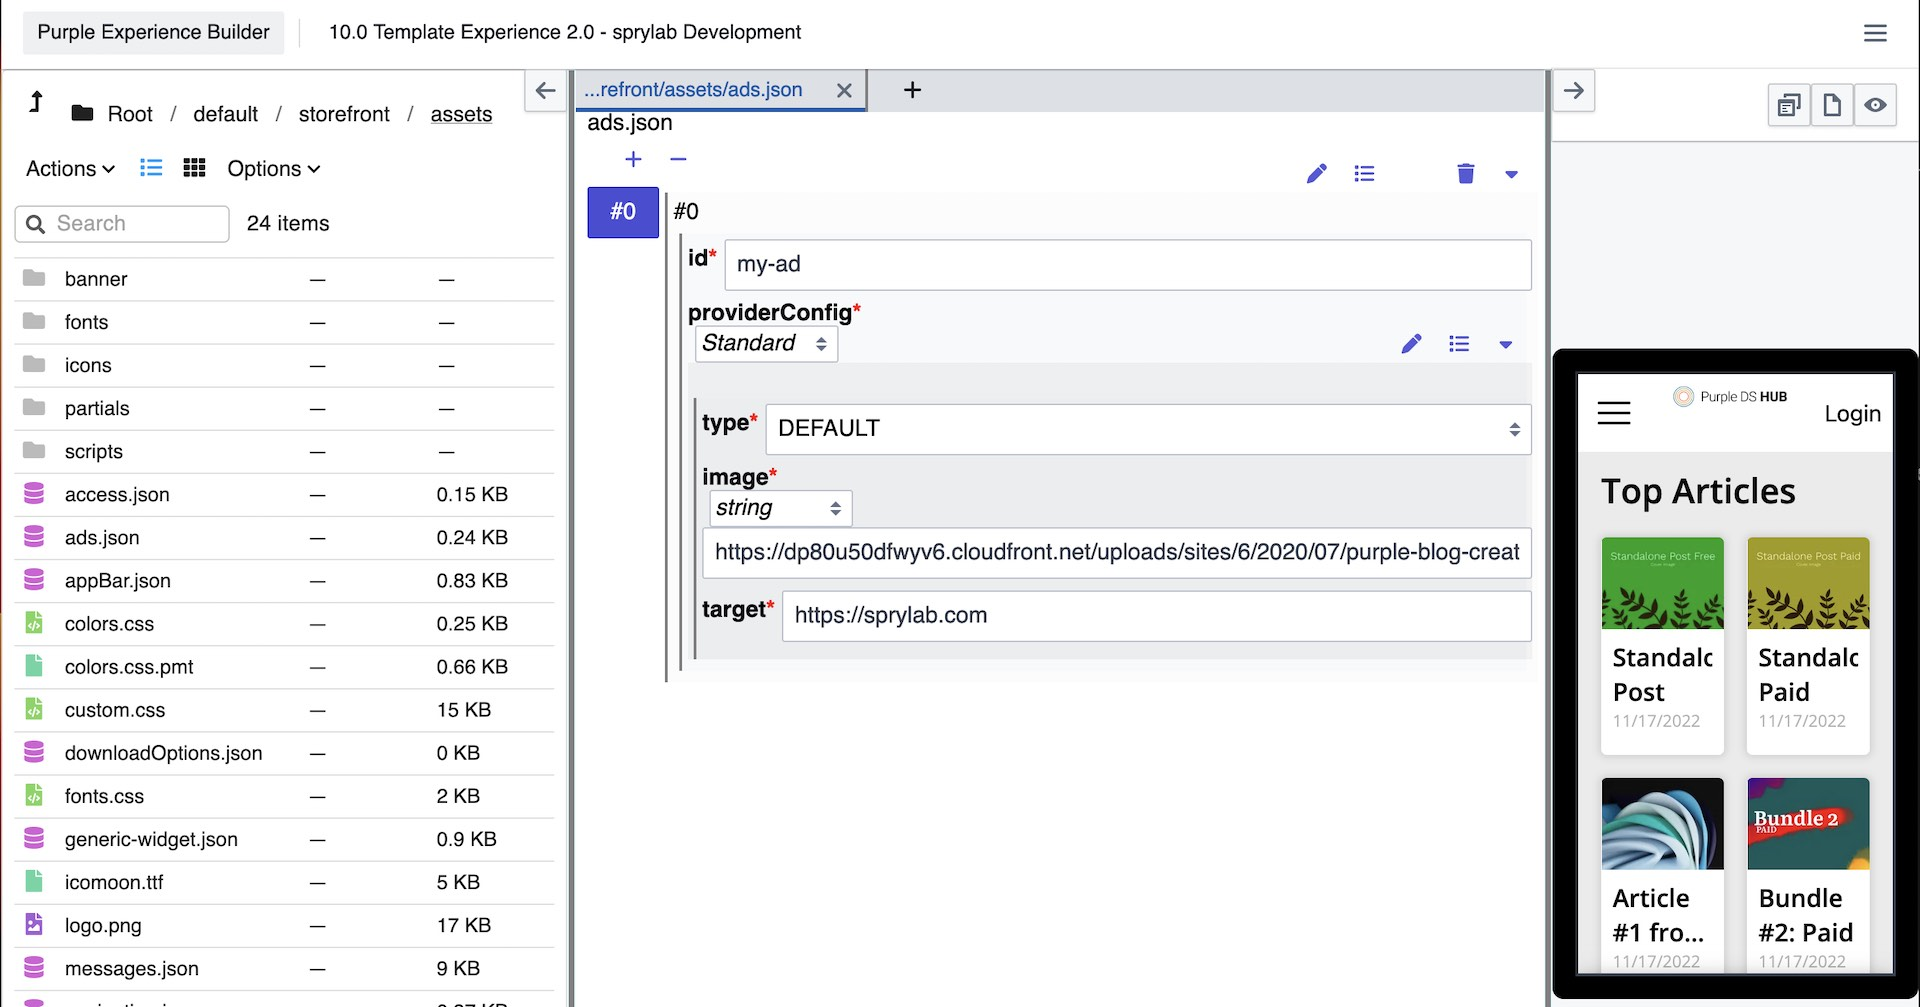
\includegraphics[width=\textwidth]{pics/ads_json_editor.jpg}
  \caption{Screenshot: JSON Editor when configuring ads}
  \label{fig:ads-editor}
\end{figure}


\section{Automated Testing}
\label{sec:automated-testing}

As already elaborated, as fast CI/CD piepline plays a crucial role for agile prototyping and development. Automated tests in turn contribute to the confidence of
developers to deploy more frequently and can reduce load from the QA team to test standard workflows every time a new release is planned.
For the Experience Builder I stuck to two of the most common testing levels: unit tests and End-to-End tests (also known as E2E or System tests).
\\\\
Unit tests are mostly used to test one ''component'' in an sandboxed environment. For the server, this meant testing Services and classes or even finer grained; single functions.
On the client, we distinguished between UI testing of single react components, and business logic code that is encapsulated in classes or Javascript modules.

They also are helpful during development to test software patterns before dogin large refactorings and to do test-driven development (TDD), where the specifications and constraints can be laid out as code
with invariants, pre- and postconditions, and then the implementation is done while continously running the tests again until they don't fail anymore.
\\
Espeically for TDD, but also for the CI/CD Pipelines, the speed of the tests is important. If a single test run takes multiple minutes, the developer is blocked during that time and can't progress on the task,
but the duration is also not long enough to start working on another task in the meantime.
That's why I tried to integrate a fast test runtime comatible with UI- / browser testing as well as node runtimes for the server code.
After evaluating diffrent commonly used frameworks, I settled for Vitest (\url{https://vitest.dev/}), which fullfills all the requirements, runs tests in parallel, thus reducing the
time between saving the change and seeing the test result to often less than a second, and has easy integration mechanisms into our build tools.
\\\\
While unit tests are a good way to verify encapsulated behaviours, when many components interact with each other, new errors can emerge often as it is
quite unrealistic to have all intenral and extenral APIs behaving exactly as expected for every input, and Web based UI applications have unmanagable number of factors that
influence the behaviour of UI, network and timings.
\\
E2E tests are supposed to cover a typical user interaction with the service to vaildate the interaction between business logic components, UI and the user itself.
I started with using a custom setup of a headless browser\footnote{Headless browsers are browser instances that don't render the actual content to a user's screen, but run as a CLI application and still execute all Javascript, CSS and HTML.} (\url{https://pptr.dev/}) in combination with vitest,
but writing and especially debugging the tests prooved slow and error prone.
\\
At an internal training day some colleagues introduced a new E2E test framework called Playwright (\url{https://playwright.dev/}), which allows recording a test case in a ''normal'' browser window, it then generates the base code for the test automatically and only needs to be adapted in a few places.
After looking through some examples and seeing how it can get integrated into our pipelines, I started porting the exisitng tests to playwright, and after a few hours the tests run on the new framework, now with much better debugging tools and the ability to add new tests much faster.
\\
This can be an example for others, that investing time to investigate new tools and port code to them if they bring value, can improve developer expeirence and thus also speed and confidence.

\section{Privacy friendly analytics \& monitoring}
\label{sec:analytics}

Sooner or later, you find yourself in a pickle when it comes to tracking.
On the one hand, the data can provide valuable insights into the behavior of many users, which would not be possible through qualitative research.
On the other hand, the most common tools like Google Analytics track users with cookies, which creates new challenges regarding GDPR compliance.
\\\\
The Purple product owner showed me a SaaS called \url{https://squeaky.ai/}, which is a cookieless solution to track users on this page.
While it can't provide the same level of demographic information a cookie based solution can, it still provides the most important data like usage statistics,
user interactions, occured Javascript errors and can even show heatmaps per page to visualize which UI elements the user interacts with the most.

\begin{figure}[h]
  \centering
  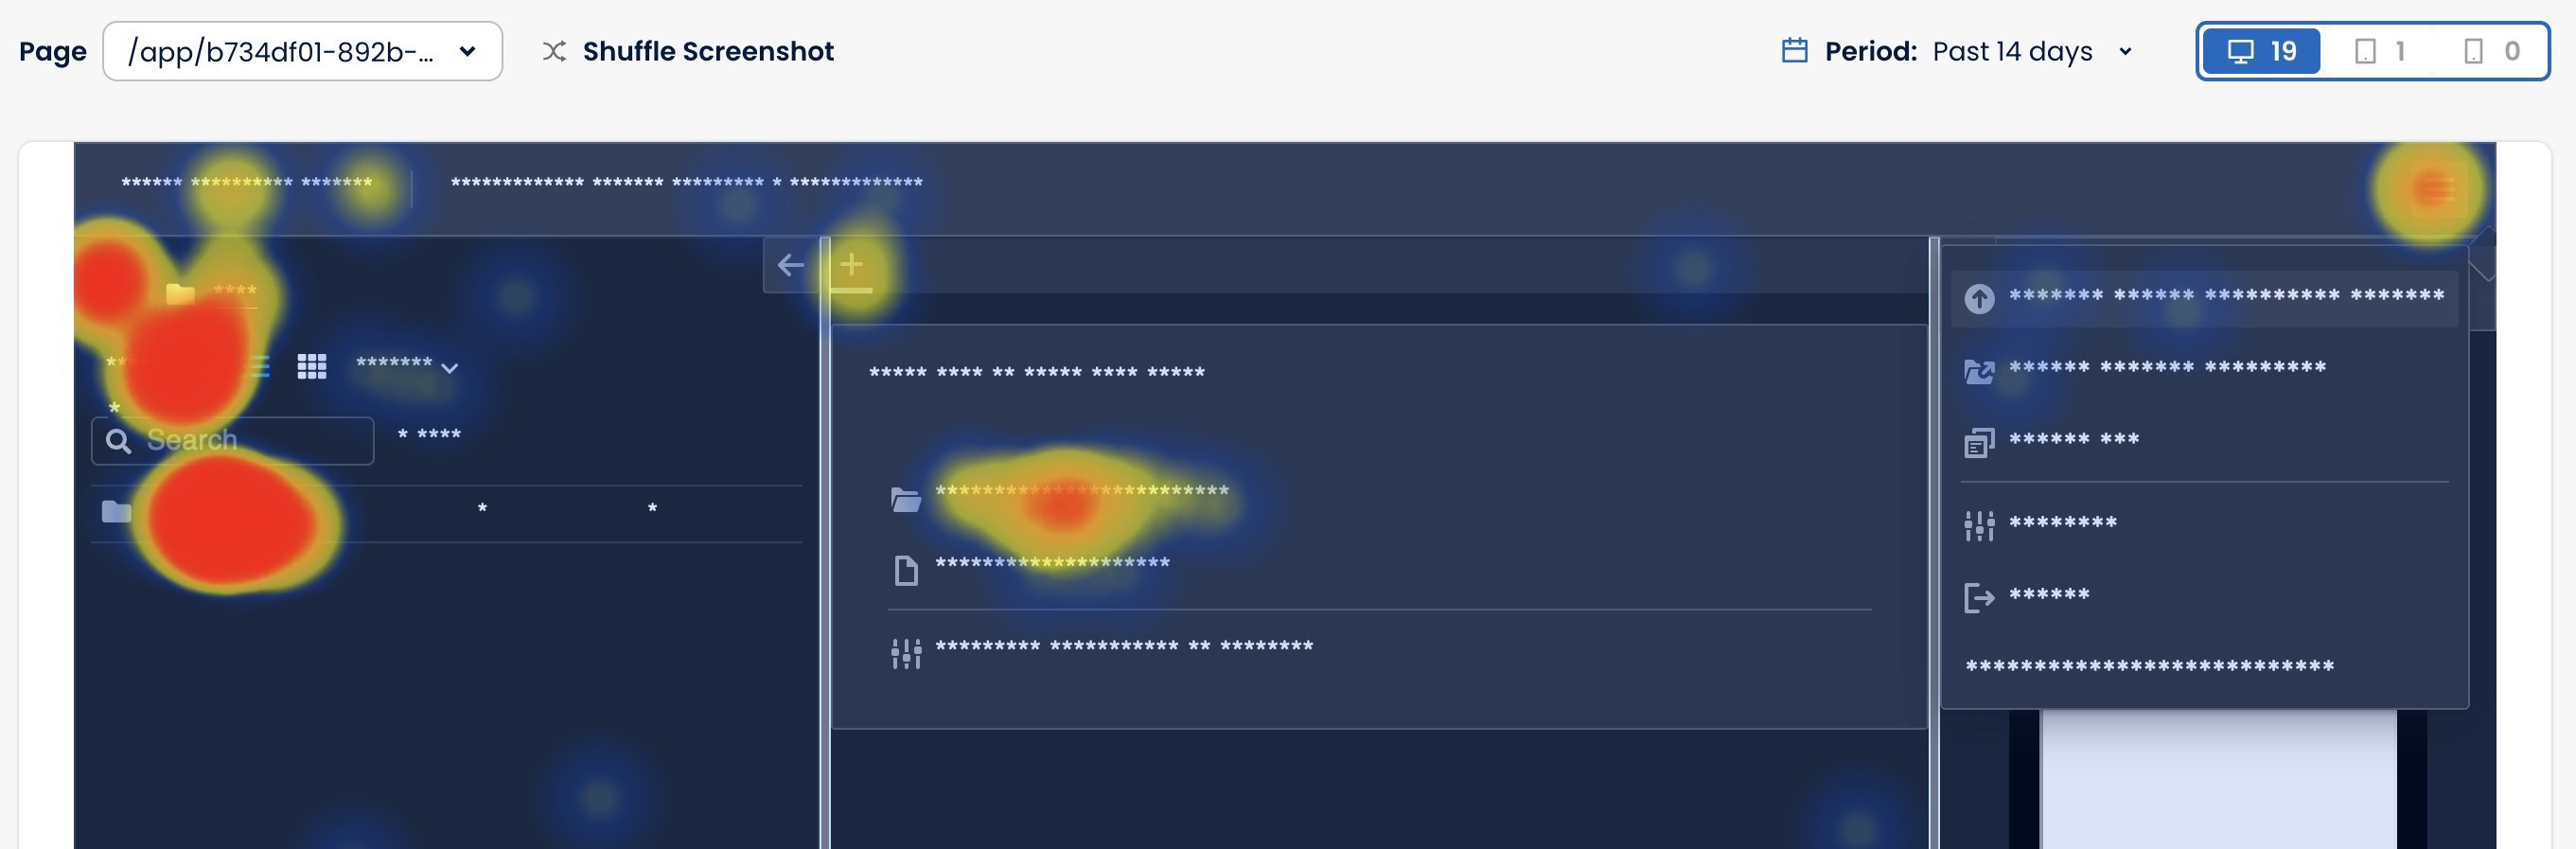
\includegraphics[width=0.75\textwidth]{pics/squeaky_heatmap.jpg}
  \caption{Screenshot: Squeaky.ai heatmap of an app's edit view}
  \label{fig:squeaky}
\end{figure}

These heatmaps for example can show if a new UI feature is used by users and how they interact with the page in general.
In case of fig. \ref{fig:squeaky}, it can be seen that the users mostly interacted with the file explorer and only did a few clicks in the editor panel.

To analyze the usage growth, fig. \ref{fig:squeaky_users} indicates how the number of page views per week increased steadily since the internal beta was started (except for the dip during the Christmas holidays).
With that graph it is save to state that the time-bound goal from the SMART goals (\ref{fig:smart}) was successfully achieved.

\begin{figure}[h]
  \centering
  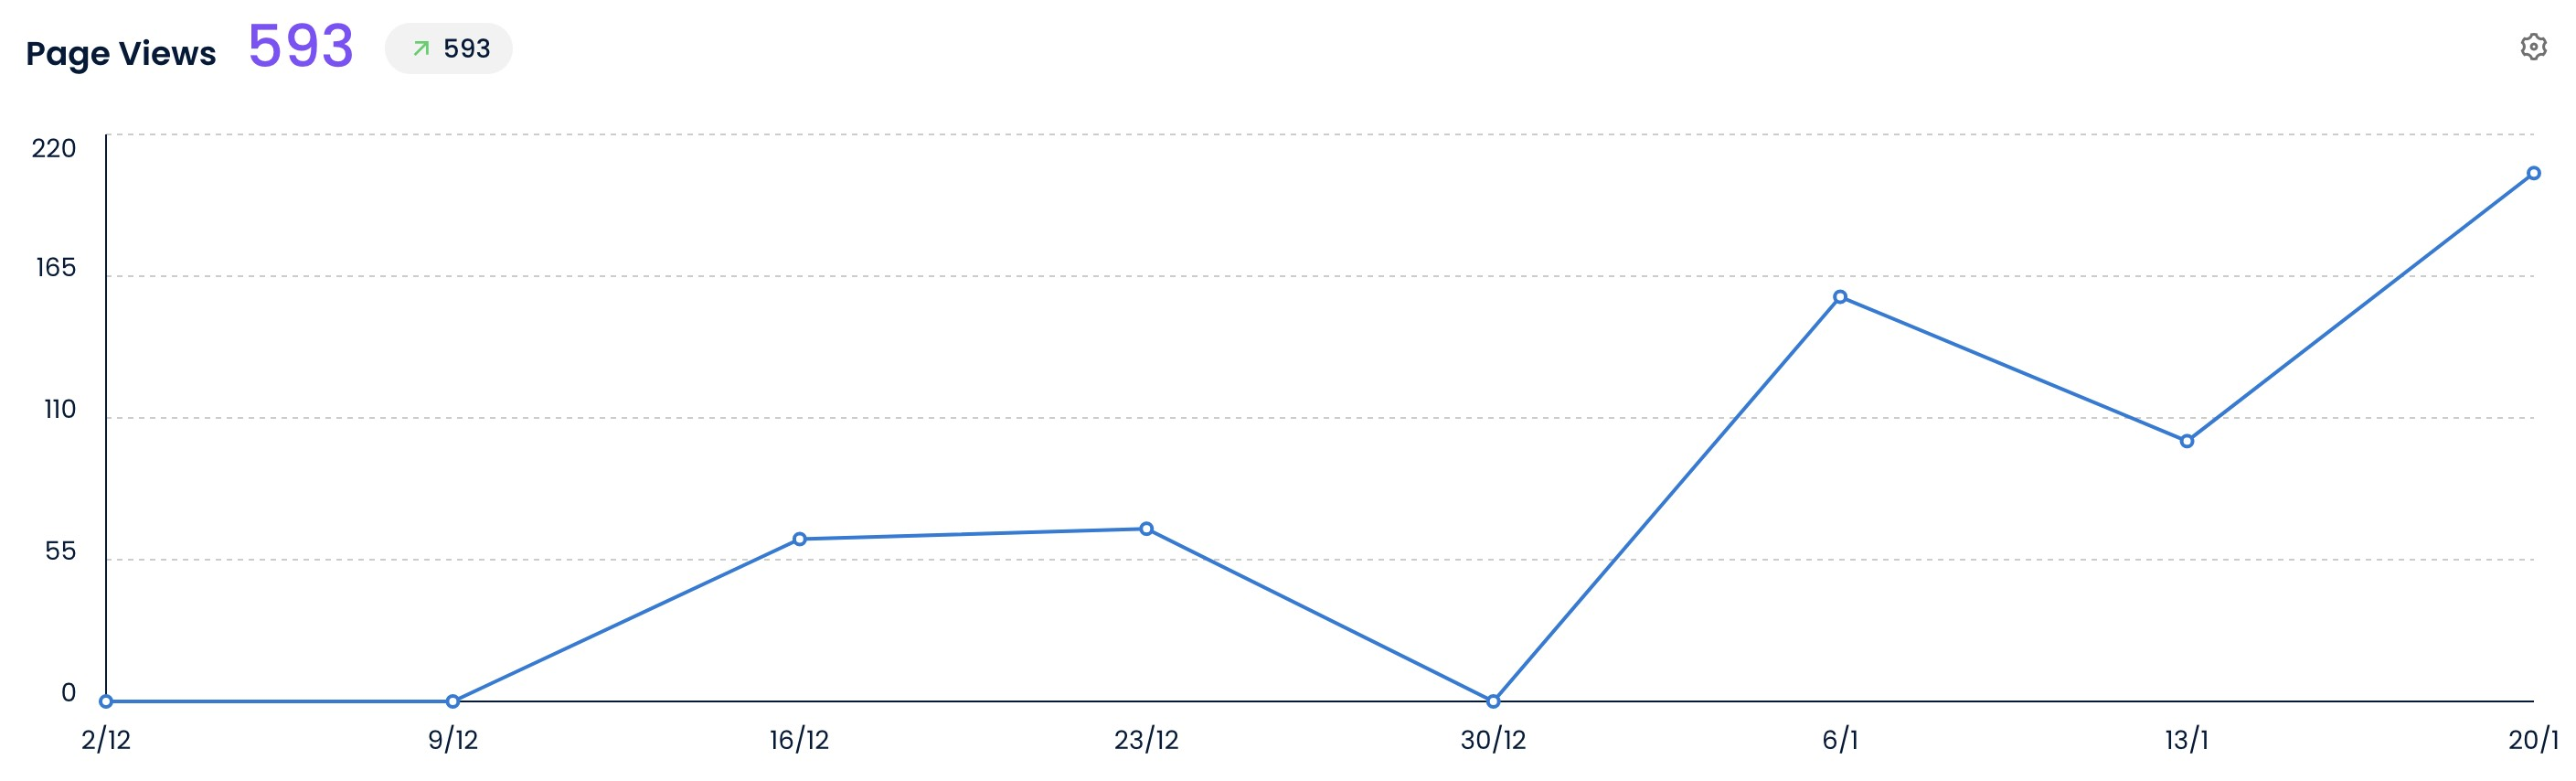
\includegraphics[width=\textwidth]{pics/squeaky_user_curve.jpg}
  \caption{Screenshot: Squeaky.ai page views since December 2022}
  \label{fig:squeaky_users}
\end{figure}

\section{User Testing, Feedback, Beta and Monitoring}

After a first stable release was done and I verified that all basic functional requirements are met and the editor doesn't destroy the dynamic resources,
I spoke with four people from our company, three of which were also interview subjects, to try to use the editor and give verbal feedback.

The reported bugs were written into Jira tickets so the status can be properly tracked and Release notes can be easier generated.
Mostly the bugs were edge cases where a file wouldn't open or the changes were not saved properly.

TODO überarbeiten

- deployments to staging
- small test group at start
- internal beta
 - problem: people didn't want to adapt new platform??
- beta flags

\section{Communication and Documentation}
Communicating with the test users and documenting the technical aspects of the software, the progress and how to use certain features is
another building block towards a good user- and developer experience.
\\
For the communication, we utilized a Microsoft Teams Channel, a group chat where all invited persons (in case of the internal bet company wide) can write with each other and create posts.
This was used for notifications about new deployments and if in the aftermath someone found a bug that could affect multiple people.

Even though this adds a bit overhead, it prooved easier than having everyone write bug tickets directly, as user often don't know the actual reason for the problem which leads to unclear descriptions, wrong tags and more.
Rather, a developer with knowledge about the system looked at the reports and created a new ticket if the problem was new, else referenced an existing ticket or forwarded the problem to the responsible team.
Jira tickets were all assigned to the UI builder component as well as specific releases so everyone can see with one click which changes and fixes are contained in which release.
\\\\
For the feature documentation, Sprylab uses Confluence for internal documentation and Archbee for external documentation that customers can access too.
As we have the common problem of documentation getting postponed indefinitely, I tried to integrate writing documentation directly int o the development flow and only close a ticket if the documentation
was written and reviewed by one additional person. Due to time and personnel shortages, this was unfortunately not always possible and will require more future attention.


% ---------------------------------------------------
% ----- Conclusion of the template
% ----- for Bachelor-, Master thesis and class papers
% ---------------------------------------------------
%  Created by C. Müller-Birn on 2012-08-17, CC-BY-SA 3.0.
%  Freie Universität Berlin, Institute of Computer Science, Human Centered Computing. 
%
\chapter{Conclusion and outlook}
\label{chap:conclusion}      
This thesis demonstrates the challenges and opportunities of applying HCI principles and methods in a brownfield software development project through the redevelopment of a UI Editor for a digital publishing company, Sprylab.
During the process, it was shown how common user research methods can be adapted to this specific case study and how technical limits and needs of users can be combined in this context.
Agile development and Lean UX enabled iterating quickly and achieving fast deployments to a staging system.
A growing group of users at Sprylab already uses the software in production.
\\\\
The consistently positive feedback shows that the chosen methods and features derived from their outcome were the right approach to enhance the user experience while complying with constraints imposed by the ecosystem.
Also, the way users were involved during the whole process led to a high level of acceptance and interest in supporting the project.
Additionally, this thesis can help to argue for the use of HCI methods in future projects started at Sprylab as well.
I'm confident that this new software is a stable and extensible tool, especially regarding the two factors Usability and Time-on-Task.
In addition to increasing user satisfaction, it also leads to enhancing productivity and customer satisfaction.

TODO: the editor enables users to safely edit JSON configurations and change assets and styles while directly seeing these changes in a preview frame
\\\\
However, there is still room for improvements in terms of accessibility and entry hurdle for new users.
The entry hurdle is still high and a lot of background knowledge is assumed, which is partly due to the complexity of other systems in the ecosystem that were set as technical requirements from the beginning on.
Moving forward, replacing the JSON editor with a custom implementation that combines JSON Schemata and generated UI is one of the next steps, which will speed up the user's
workflow even more and allow for further improvements that are impossible with a third-party library.
\\\\
Overall, this thesis has demonstrated the importance of considering HCI principles and methods in brownfield software development projects, and the potential benefits that can be achieved when these approaches are applied in a real-world context.


%---------------------------------------------------
%----- Bibliography
%---------------------------------------------------
\phantomsection
\addcontentsline{toc}{chapter}{Bibliography}
% \bibliographystyle{alpha}
\printbibliography

%---------------------------------------------------
%----- Appendix   
%---------------------------------------------------
\backmatter
\printnoidxglossaries
% ---------------------------------------------------
% ----- Appendix of the template
% ----- for Bachelor-, Master thesis and class papers
% ---------------------------------------------------
%  Created by C. Müller-Birn on 2012-08-17, CC-BY-SA 3.0.
%  Freie Universität Berlin, Institute of Computer Science, Human Centered Computing. 
%

\chapter{Appendix}
\label{ch:Appendix}

\section{Erster Teil Appendix}
\label{app:first_appendix} 

\section{Zweiter Teil Appendix}
\label{app:second_appendix}  



\end{document}